% CVPR 2025 Paper Template; see https://github.com/cvpr-org/author-kit

\documentclass[10pt,twocolumn,letterpaper]{article}

%%%%%%%%% PAPER TYPE  - PLEASE UPDATE FOR FINAL VERSION
\usepackage{cvpr}              % To produce the CAMERA-READY version
% \usepackage[review]{cvpr}      % To produce the REVIEW version
% \usepackage[pagenumbers]{cvpr} % To force page numbers, e.g. for an arXiv version

% Import additional packages in the preamble file, before hyperref
%
% --- inline annotations
%
\newcommand{\red}[1]{{\color{red}#1}}
\newcommand{\todo}[1]{{\color{red}#1}}
\newcommand{\TODO}[1]{\textbf{\color{red}[TODO: #1]}}
% --- disable by uncommenting  
% \renewcommand{\TODO}[1]{}
% \renewcommand{\todo}[1]{#1}

\usepackage{xcolor}
\usepackage{graphicx}
\usepackage{booktabs}
\usepackage{amsmath} 
\usepackage{amsfonts}
\usepackage{amssymb}
\usepackage{multirow} 
\usepackage{makecell}
\newcommand{\shline}{\Xhline{1.1pt}} % Adjust thickness as desired

% It is strongly recommended to use hyperref, especially for the review version.
% hyperref with option pagebackref eases the reviewers' job.
% Please disable hyperref *only* if you encounter grave issues, 
% e.g. with the file validation for the camera-ready version.
%
% If you comment hyperref and then uncomment it, you should delete *.aux before re-running LaTeX.
% (Or just hit 'q' on the first LaTeX run, let it finish, and you should be clear).
\definecolor{cvprblue}{rgb}{0.21,0.49,0.74}
\usepackage[pagebackref,breaklinks,colorlinks,allcolors=cvprblue]{hyperref}

%%%%%%%%% PAPER ID  - PLEASE UPDATE
\def\paperID{6709} % *** Enter the Paper ID here
\def\confName{CVPR}
\def\confYear{2025}

%%%%%%%%% TITLE - PLEASE UPDATE
\title{\dataset: Learning How Things Move in 3D from Internet Stereo Videos}

%%%%%%%%% AUTHORS - PLEASE UPDATE

\author{
Linyi Jin$^{1,2}$\qquad
Richard Tucker$^1$\qquad
Zhengqi Li$^1$\qquad
David Fouhey$^3$\\
Noah Snavely$^{1*}$\qquad
Aleksander Holynski$^{1*}$
\\[0.5em]
$^1$Google DeepMind \ \ \
$^2$University of Michigan \ \ \ 
$^3$New York University \ \ \ 
$^*$equal contribution\\ \\
}

\begin{document}
\twocolumn[{%
\renewcommand\twocolumn[1][]{#1}%
\maketitle
\vspace{-2em}
 \includegraphics[width=\textwidth]{fig/teaser_v5.pdf}
\captionof{figure}{There is currently no scalable source of data for real-world, ground truth 3D motion paired with video. 
We present a framework for mining such data from existing stereoscopic videos on the Internet, in the form of 3D point clouds with long-range world-space trajectories. Our framework fuses and filters camera poses, dense depth maps, and 2D motion trajectories to produce high-quality, pseudo-metric point clouds with long-term 3D motion trajectories, pictured above, for hundreds of thousands of video clips. We show how this data is useful in learning a model that reasons about both 3D shape and motion in imagery.\\ }
\label{fig:teaser}
}]
\begin{abstract}
Segment Anything Model 2 (SAM 2) has emerged as a powerful tool for video object segmentation and tracking anything. Key components of SAM 2 that drive the impressive video object segmentation performance include a large multistage image encoder for frame feature extraction and a memory mechanism that stores memory contexts from past frames to help current frame segmentation. The high computation complexity of multistage image encoder and memory module has limited its applications in real-world tasks, e.g., video object segmentation on mobile devices. To address this limitation, we propose EfficientTAMs, lightweight track anything models that produce high-quality results with low latency and model size. Our idea is based on revisiting the plain, nonhierarchical Vision Transformer (ViT) as an image encoder for video object segmentation, and introducing an efficient memory module, which reduces the complexity for both frame feature extraction and memory computation for current frame segmentation. We take vanilla lightweight ViTs and efficient memory module to build EfficientTAMs, and train the models on SA-1B and SA-V datasets for video object segmentation and track anything tasks. We evaluate on multiple video segmentation benchmarks including semi-supervised VOS and promptable video segmentation, and find that our proposed EfficientTAM with vanilla ViT perform comparably to SAM 2 model (HieraB+SAM 2) with $\sim$2x speedup on A100 and $\sim$2.4x  parameter reduction. On segment anything image tasks, our EfficientTAMs also perform favorably over original SAM with $\sim$20x  speedup on A100 and $\sim$20x  parameter reduction. On mobile devices such as iPhone 15 Pro Max, our EfficientTAMs can run at $\sim$10 FPS for performing video object segmentation with reasonable quality, highlighting the capability of small models for on-device video object segmentation applications. 
\end{abstract}    
\section{Introduction}
Deep learning techniques have made rapid progress in conditional image generation. For example, networks have been used to inpaint missing image regions~\citep{pathakCVPR16context,yang2016high,isola2016image}, 
add color to grayscale images~\citep{iizuka2016let,larsson2016learning,zhang2016colorful,isola2016image}, and generate photorealistic images from sketches~\cite{sangkloy2017scribbler,isola2016image}.
However, most techniques in this space have focused on generating a \textit{single} result.
In this work, we model a \textit{distribution} of potential results, as many of these problems may be multimodal in nature. For example,
as seen in Figure~\ref{fig:teaser}, an image captured at night may look very different in the day, depending on cloud patterns and lighting conditions.
We pursue two main goals: producing results which are (1) perceptually realistic and (2) diverse, all while remaining faithful to the input.

Mapping from a high-dimensional input to a high-dimensional output distribution is challenging. A common approach to representing multimodality is learning a low-dimensional latent code, which should represent aspects of the possible outputs not contained in the input image. At inference time, a deterministic generator uses the input image, along with stochastically sampled latent codes, to produce randomly sampled outputs. A common problem in existing methods is~\textit{mode collapse}~\citep{goodfellow2016nips}, where only a small number of real samples get represented in the output.
We systematically study a family of solutions to this problem.

We start with the \pp framework~\citep{isola2016image}, which has previously been shown to produce high-quality results for various image-to-image translation tasks. The method trains a generator network, conditioned on the input image, with two losses: (1) a regression loss to produce similar output to the known paired ground truth image and (2) a learned discriminator loss to encourage realism. The authors note that trivially appending a randomly drawn latent code did not produce diverse results. Instead, we propose encouraging a bijection between the output and latent space. 
We not only perform the direct task of mapping the latent code (along with the input) to the output but also jointly learn an encoder from the output back to the latent space. 
This discourages two different latent codes from generating the same output (non-injective mapping).
During training, the learned encoder attempts to pass enough information to the generator to resolve any ambiguities regarding the output mode.
For example, when generating a day image from a night image, the latent vector may encode information about the sky color, lighting effects on the ground, and cloud patterns.  Composing the encoder and generator sequentially should result in the same image being recovered. The opposite should produce the same latent code.

\begin{figure}
\centering
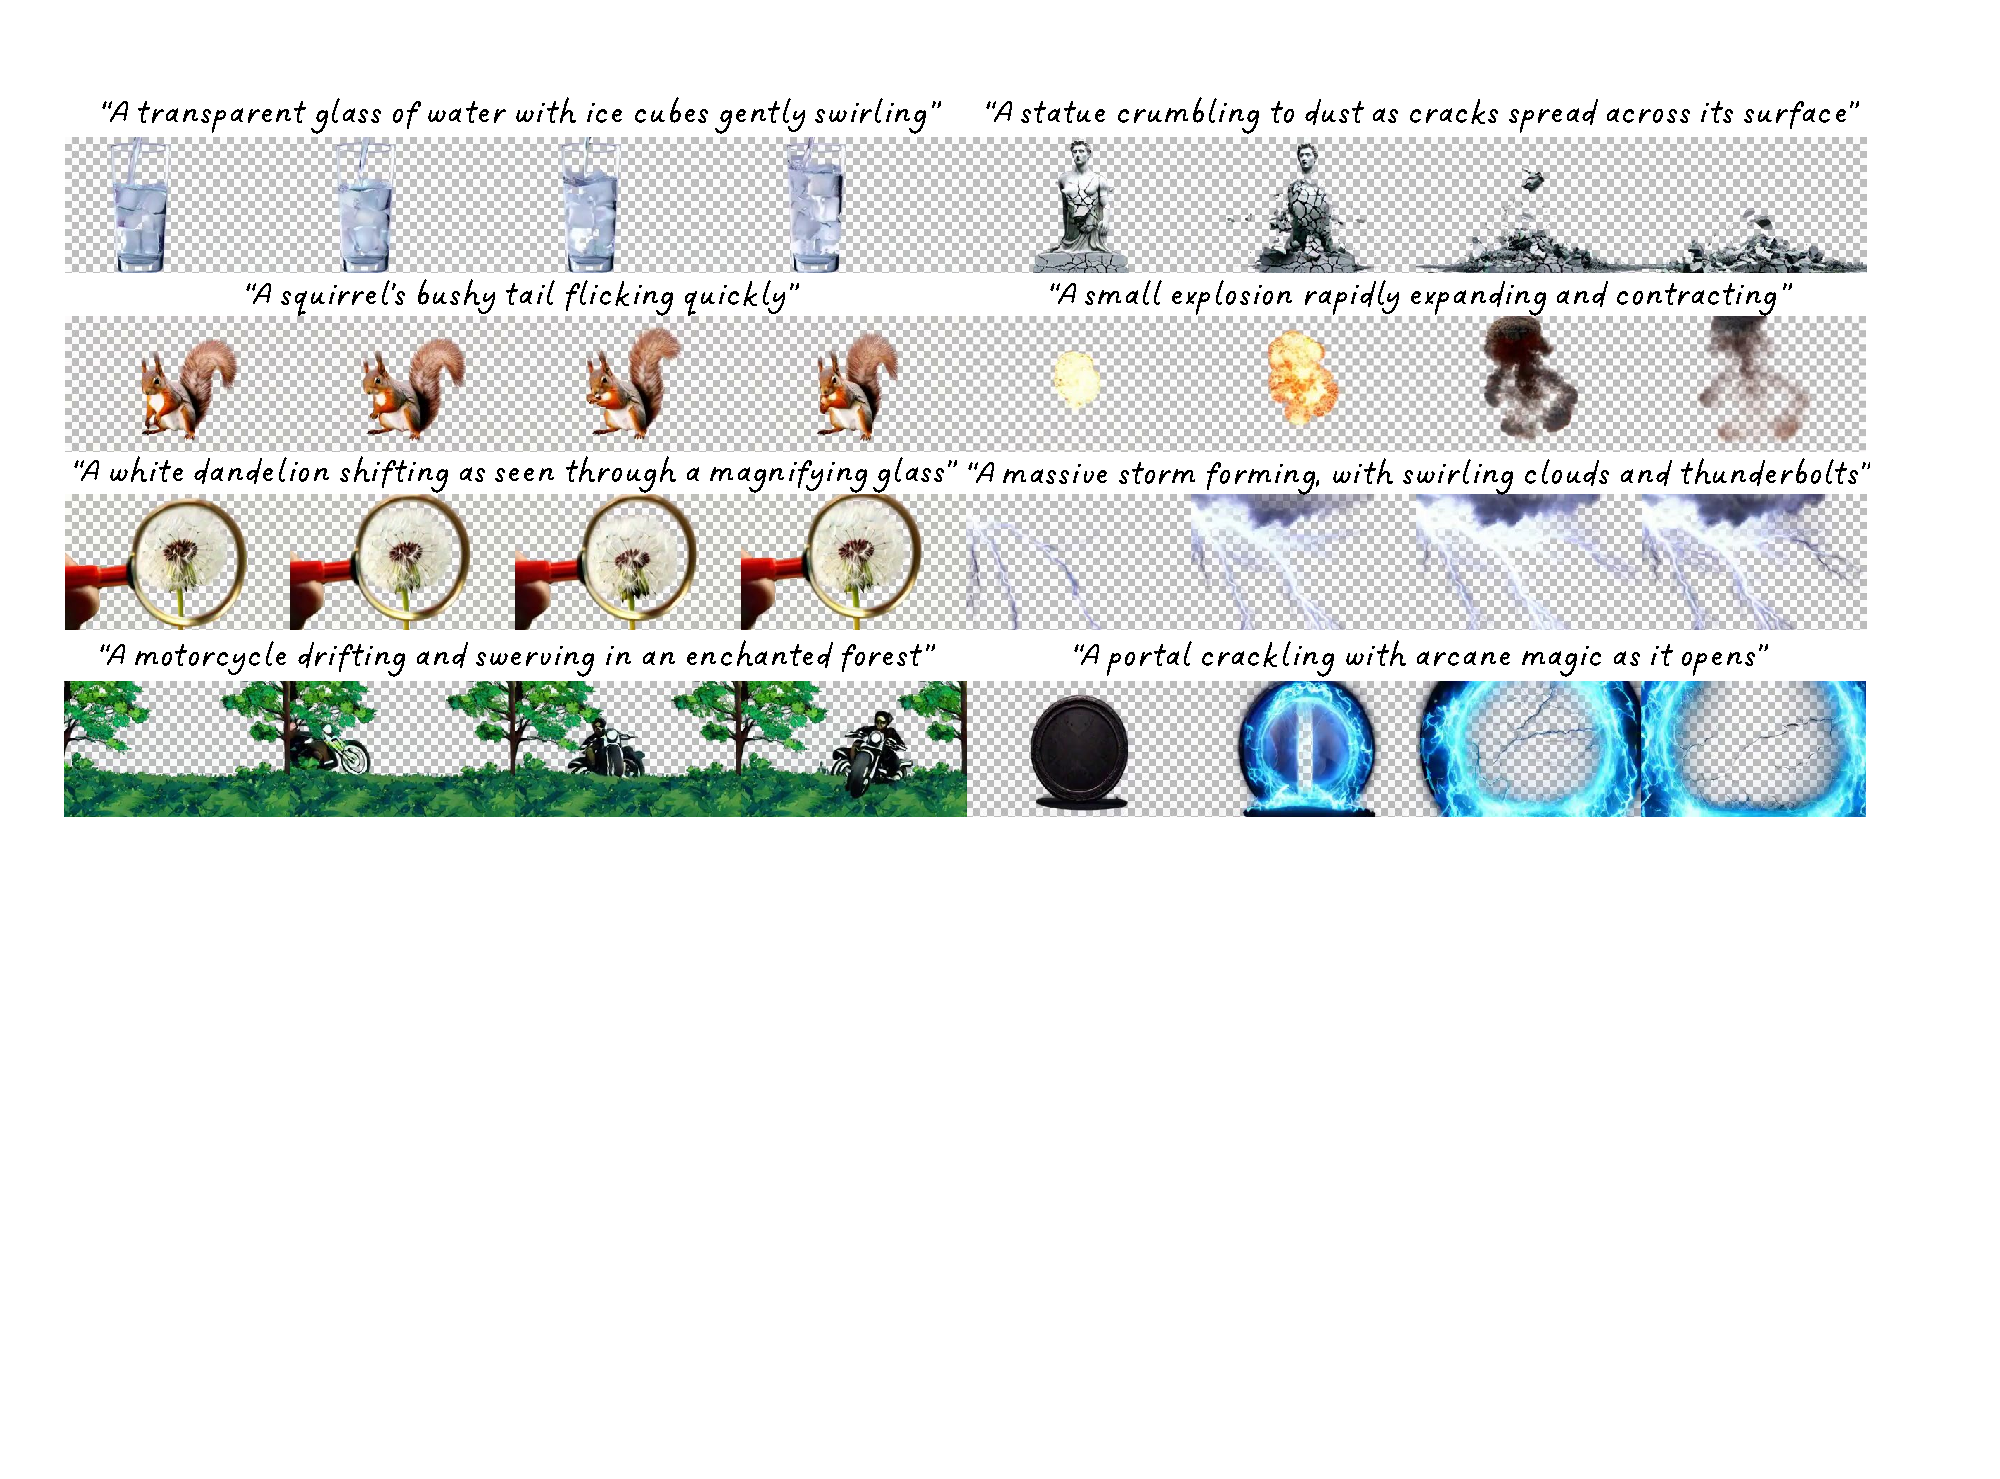
\includegraphics[width=1.\linewidth]{imgs/teaser.pdf}
\vspace{-4mm}
\caption{\small Multimodal image-to-image translation using our proposed method: given an input image from one domain (night image of a scene), we aim to model a \textit{distribution} of potential outputs in the target domain (corresponding day images), producing both realistic and diverse results.}
\vspace{-4mm}
\label{fig:teaser}
\end{figure}


In this work, we instantiate this idea by exploring several objective functions, inspired by literature in unconditional generative modeling:
  \begin{itemize}[leftmargin=0.1in]
  
    \item \textbf{\cvaegan (Conditional Variational Autoencoder GAN)}:
    One approach is first encoding the ground truth image into the latent space, giving the generator a noisy ``peek" into the desired output. Using this, along with the input image, the generator should be able to reconstruct the specific output image. To ensure that random sampling can be used during inference time, the latent distribution is regularized using KL-divergence to be close to a standard normal distribution. This approach has been popularized in the unconditional setting by VAEs~\citep{kingma2013auto} and VAE-GANs~\citep{larsen2016vaegan}.
    
    \item \textbf{\cinfogan (Conditional Latent Regressor GAN)}: Another approach is to first provide a randomly drawn latent vector to the generator. In this case, the produced output may not necessarily look like the ground truth image, but it should look realistic. An encoder then attempts to recover the latent vector from the output image. This method could be seen as a conditional formulation of the ``latent regressor" model~\citep{donahue2016adversarial,dumoulin2016adversarially} and also related to InfoGAN~\citep{xi2016infogan}.
    
    \item \textbf{\bicycle}: Finally, we combine both these approaches to enforce the connection between latent encoding and output in both directions {\em jointly} and achieve improved performance. We show that our method can produce both diverse and visually appealing results across a wide range of image-to-image translation problems, significantly more diverse than other baselines, including naively adding noise in the \pp framework. In addition to the loss function, we study the performance with respect to several encoder networks, as well as different ways of injecting the latent code into the generator network. 
\end{itemize}

We perform a systematic evaluation of these variants by using humans to judge photorealism and a perceptual distance metric~\cite{zhang2018unreasonable} to assess output diversity. Code and data are available at \url{https://github.com/junyanz/BicycleGAN}.
\section{Related Works}
\label{sec:related}

\textbf{Diffusion Models}.
Diffusion models \cite{sohl2015deep, song0, ddpm} decompose the image generation task into a sequence of iterative denoising steps, gradually transforming noise into a coherent image. Early diffusion models \cite{adm, rombach2022high, sdxl, nichol2021glide, dalle2} with U-net architectures pioneered denoising techniques for high-quality image synthesis. Later works \cite{dit, bao2023all} like DiT shift from the U-net to transformer-based architectures, enabling greater compute scalability. Modern methods \cite{, chen2024pixart, flux} further extend DiT architectures leveraging significantly larger training resources to achieve impressive image generation quality.

\vspace{3pt}
\textbf{Autoregressive Generation}.
Another popular approach for image generation involves autoregressive (AR) transformers that predict images token by token. Early works \cite{dalle1, ding2021cogview, gafni2022make, parti} generated image tokens in raster order, progressing sequentially across the image grid. This rasterized approach was later identified as inefficient \cite{chang2022maskgit}, prompting researchers to explore random-order generation methods \cite{chang2022maskgit, muse}. 
AR methods are further evolved to include new modalities such as video generation~\cite{kondratyukvideopoet} and any-to-any generation~\cite{io2, anygpt}. 

\vspace{3pt}
\textbf{Combining Diffusion and Autoregressive Models}.
Recent models explore different methods for integrating AR and diffusion processes. DART \cite{dart} unifies AR and diffusion in a non-Markovian framework by conditioning on multiple historical denoising steps instead of only the current one. BiGR \cite{bigr} generates discrete binary image codes autoregressively using a Bernoulli diffusion process. MAR \cite{mar} employs an AR model with a small diffusion head to enable continuous-value generation. Emu2 \cite{emu2} applies an external diffusion module to decode its AR-based multimodal outputs. 
Compared to previous methods, CausalFusion focuses on autoregressive sequence factorization and decouples diffusion data processing across both sequential tokens and noise levels, achieving significant performance gains over traditional diffusion frameworks.


\section{Creating a dataset of 4D scenes}
\label{sec:data}


\begin{figure}
    \centering
    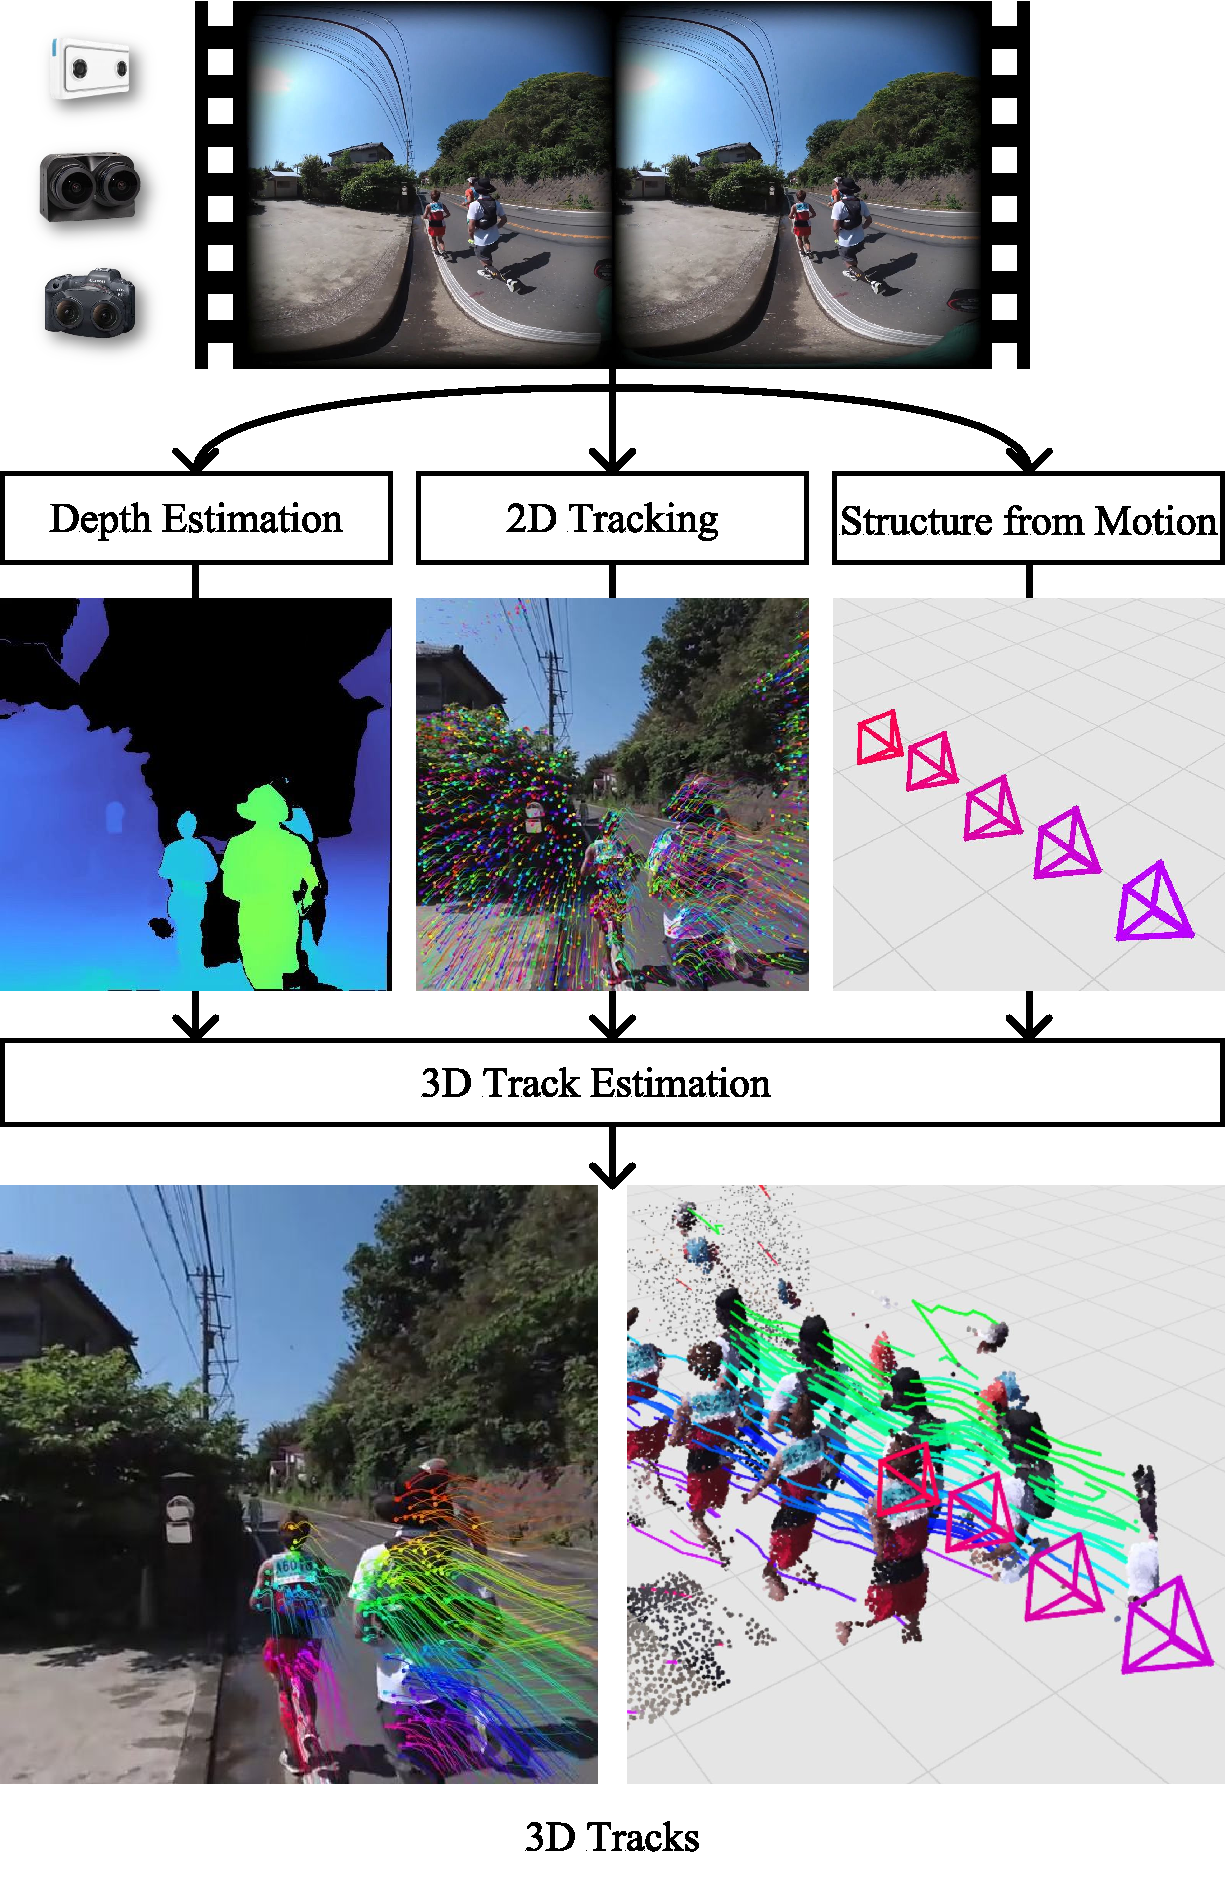
\includegraphics[width=\linewidth]{fig/data_processing_vertical.pdf}
    \vspace{-2em}
    \caption{\textbf{Data processing pipeline.} Our method starts with VR180 (wide-angle, stereoscopic) videos, and estimates metric stereo depth, 2D point tracks, and camera poses. These quantities allow the tracks to be lifted to 3D where they are filtered and denoised to produce world-space, metric 3D point trajectories.}
    \label{fig:data_pipeline}
\end{figure}

A core contribution of this work is a pipeline for extracting high-quality, pseudo-metric, 3D data from online stereoscopic fisheye videos (known as VR180 videos). 
High-resolution, wide field of view VR180 videos can be found readily online.
We show that this data is ideal for deriving rich dynamic 3D information that can power models for predicting geometry and motion from imagery.

Concretely, each instance of data starts as an $N$ frame stereo video consisting of left-right image pairs $\IB_i$ and $\IB'_i$ indexed by frame index $i\in[1,N]$. We convert these stereo pairs to a dynamic 3D point cloud with $K$ points in a world-space coordinate frame, where each point, indexed by $j\in[1,K]$, has a time-varying position $\pB_i^j$. 
As part of the process of generating this dynamic point cloud, we also extract a number of auxiliary quantities: (1) per-frame camera extrinsics, (the left camera's position $\cB_i$ and orientation $\RB_i$), (2) rig calibration for the stereo video giving the position $\cB_r$ and orientation $\RB_r$ of the right camera relative to the left camera, and (3) a per-frame disparity map $\DB_i$.


\subsection{Data Processing Pipeline} 

At a high level, our pipeline for converting a stereoscopic video into a dynamic point cloud involves estimating camera poses, stereo disparity, and 2D tracks, fusing these quantities into a consistent 3D coordinate frame, and performing several filtering operations to ensure temporal consistent, high-quality reconstructions (\Fig{data_pipeline}). In this section, we describe in detail the key components of this process. %


\medskip
\noindent \textbf{SfM.} 
We start by processing the sequence of stereo frames $\IB_i \leftrightarrow \IB_i'$ to produce camera pose estimates ($\cB_i, \RB_i$). We first use a SLAM method to divide the video into shots, as in~\cite{zhou2017scene}. For each shot, we run an incremental SfM algorithm similar to COLMAP~\cite{schonberger2016structure}. We initialize the stereo rig calibration $(\cB_r, \RB_r)$ to a rectified stereo pair with baseline $6.3$cm, but optimize for the calibration in bundle adjustment. In practice, we found that the exact stereo pair orientation can vary significantly from its nominal configuration and that optimizing the rig was critical for good results. 

\medskip 
\noindent \textbf{Depth Estimation.}
We next estimate a per-frame disparity map, operating on each frame independently. In particular, we use the estimated camera rig calibration $\cB_r, \RB_r$ to create rectified stereo pairs from the stereo fisheye video and estimate the per-frame disparity~$\DB_i$ with RAFT~\cite{sun2022disentangling,
sun2021autoflow,teed2020raft}. 

\medskip
\noindent \textbf{3D Track Estimation and Optimization.}  %
We extract long-range 2D point trajectories using BootsTAP~\cite{doersch2024bootstap}. Using the camera poses $\cB_i, \RB_i$ and disparity maps $\DB_i$, we unproject these tracked points into 3D space, turning each 2D track $j$ into a 3D motion trajectory $\pB^j_1, \ldots, \pB^j_N$
 across all frames. In general, each point will usually only be tracked in a subset of frames, but for simplicity, we describe the formulation as if all points are always visible. Moreover, since subsequent steps are done independently per-track, we drop the superscript $j$ in future references. 

Since stereo depth estimation is performed per-frame, the initial disparity estimates (and therefore, the 3D track positions) are likely to exhibit high-frequency temporal jitter. To compensate for potentially inconsistent disparity estimates, we formulate an optimization strategy that solves for a per-frame scalar offset $\delta_i \in \mathbb{R}$ that moves each point $\pB_i$ along the ray from camera location $\cB_i$ to $\pB_i$ at frame $i$. 
This ray is denoted $\rB_i = (\pB_i - \cB_i) / ||\pB_i - \cB_i||$, and we refer to the updated location as $\pB_i' = \pB_i + \delta_i \rB_i$. 

To ensure static points remain stationary while moving tracks maintain realistic, smooth motion, avoiding abrupt depth changes frame by frame, we design an optimization objective comprising three terms: a static loss $\mathcal{L}_{\mathsf{static}}$, a dynamic loss $\mathcal{L}_{\mathsf{dynamic}}$, and a regularization loss $\mathcal{L}_{\mathsf{reg}}$. The static loss $\mathcal{L}_{\mathsf{static}}$ minimizes jitter by encouraging points to remain close to each other in world space:
\begin{equation}
\mathcal{L}_{\mathsf{static}} = \sum_{i=1}^{N} \sum_{j=1}^{N} \frac{\| \mathbf{p}_i' - \mathbf{p}_j' \|^2}{N_p'^2}
\label{eq:objective_function}
\end{equation}
where $N_p' = \sum_{i=1}^N{\|\mathbf{p}'_i\|} / N$ is a normalizing factor.
The dynamic loss term reduces jitter by minimizing acceleration along the camera ray through a discrete Laplacian operator:
\begin{equation}
\mathcal{L}_{\mathsf{dynamic}} = \sum_{i=1}^{N} \sum_{\Delta\in\mathcal{W}} \left[ \left( \mathbf{p}_{i+\Delta}' - 2\mathbf{p}_i' + \mathbf{p}_{i-\Delta}' \right)^\top \mathbf{r}_i \right]^2
\label{eq:dynamic_objective}
\end{equation}
where the acceleration along the ray is calculated over
multiple window sizes $\mathcal{W}=\{1,3,5\}$.


The two loss terms are weighted by a track-dependent function, $\sigma(m)$, where $m$ is a measure of the motion magnitude of the track. Motion is measured in 2D rather than 3D because distant points can appear to have a larger 3D motion due to noise amplification at low disparities.
Specifically, we project the 3D motion trajectory between time $i - w_o$ and the current time $i$ into 2D image-space at time $i$, %
and calculate the track's motion magnitude $m$ as the 90$^{th}$ percentile of the track's trail length across all frames. The track trail length for a frame is measured by projected 3D points along the track to the current frame as if the camera is \emph{static} in a window of $w_o=16$ frames, 
\begin{equation}
\label{eqn:trail_length_def}
    m = \mathsf{Percentile}_{i=1:N}^{90}\left[\max_{w=1:w_o}\|\pi_i(\pB_i) - \pi_i(\pB_{i-w})\|\right]
\end{equation}
where $\pi_i(\cdot)\in \mathbb{R}^2$ gives the projected pixel location of a 3D point on camera $\cB_i$'s image plane.
The weighting function $\sigma(m)$ is defined as $\sigma(m) = \frac{1}{1 + \exp(m - m_0)}$ where $m_0 = 20$. 
Finally, to encourage faithfulness to the originally estimated disparities, we regularize the displacements in disparity space:
\begin{equation}
    \mathcal{L}_{\mathsf{reg}} = \lambda_{\mathsf{reg}} \sum_{i=1}^{T} \left( \frac{1}{\delta_i + \|\mathbf{p}_i-\mathbf{c}_i\|} - \frac{1}{\|\mathbf{p}_i-\mathbf{c}_i\|} \right)^2,
\end{equation}
where use of disparity space reflects the fact that the measurements themselves originate as disparities. Practically, the impact of the use of disparity is that larger deviations are tolerated at more distant points, where depth is intrinsically more uncertain.

The full objective function is
\begin{equation}
\min_{\{\delta_i\}_{i=1}^N} \sigma(m)\mathcal{L}_{\mathsf{static}} + (1-\sigma(m))\mathcal{L}_{\mathsf{dynamic}} + \mathcal{L}_{\mathsf{reg}}.
\label{eqn:objective}
\end{equation}
We set $\lambda_{\mathsf{reg}}=10^{-4}$ and optimize Eqn.~\ref{eqn:objective} using Adam with a learning rate of 0.05 for 100 steps.
The effect of track optimization is shown in \Fig{track_optimization}. The optimized motion is smoother and does not contain high frequency noise.


\begin{figure}[t]
    \centering
    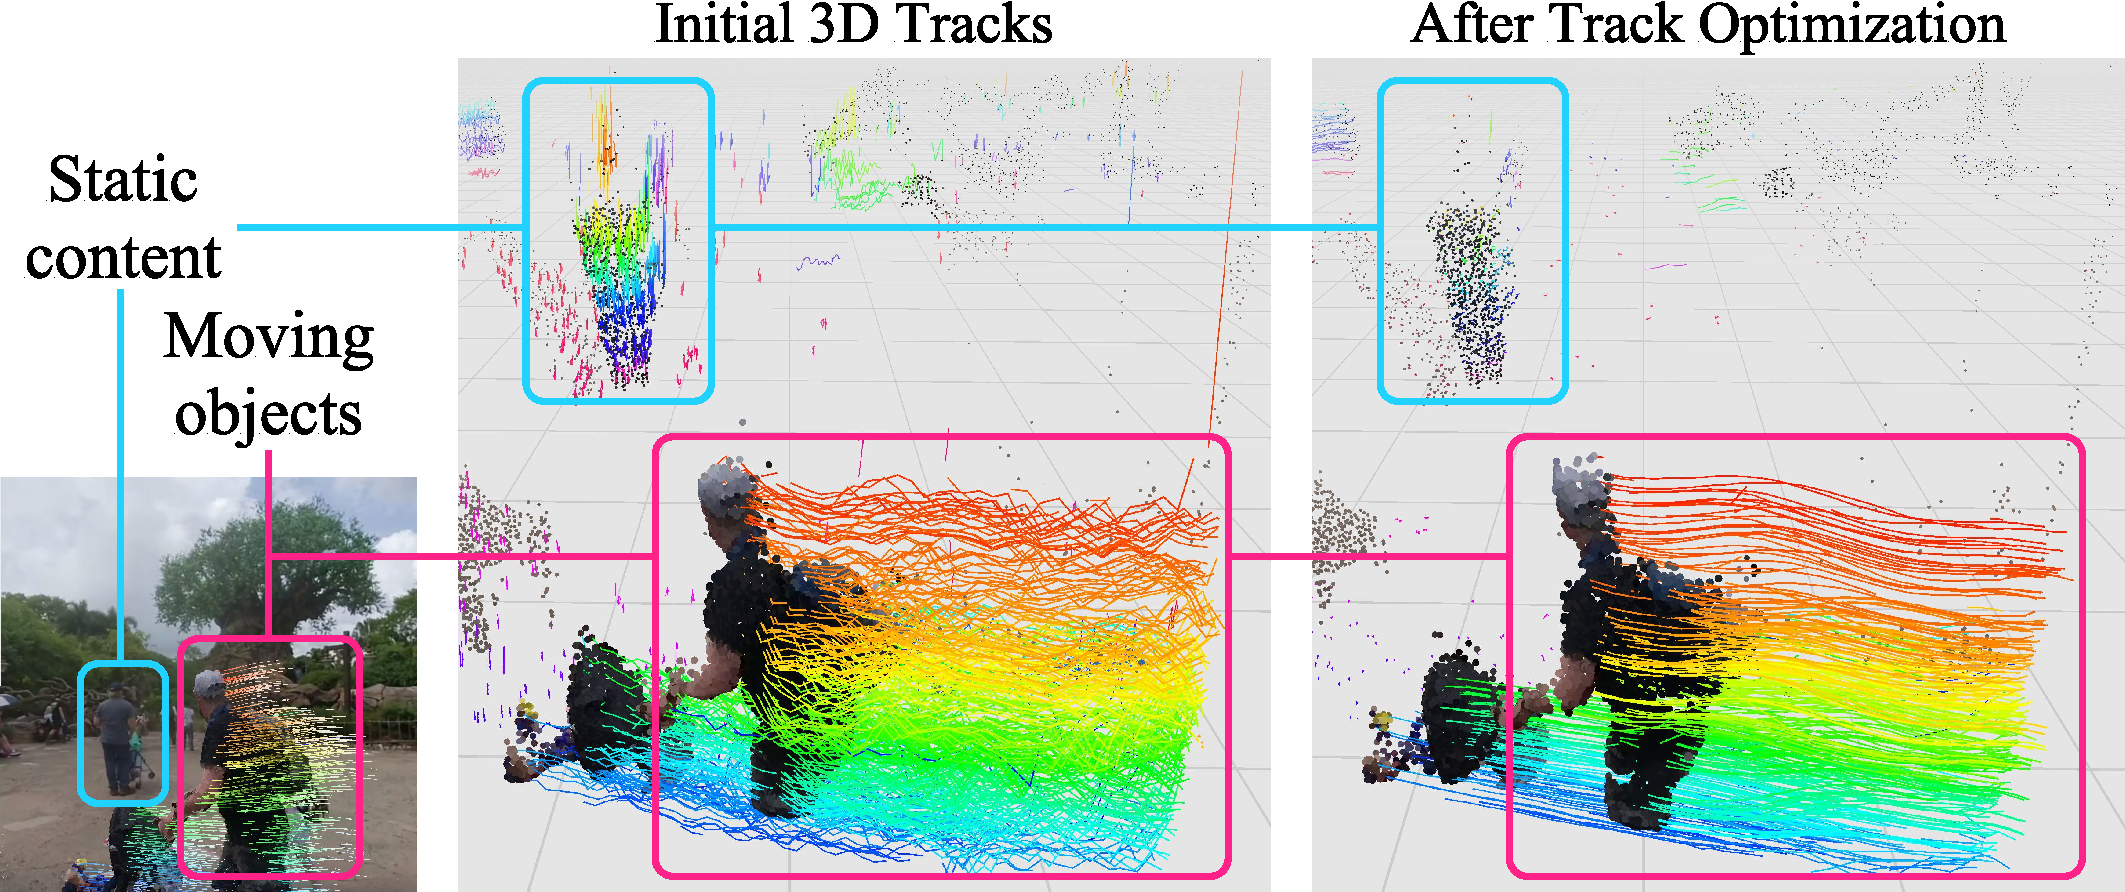
\includegraphics[width=\linewidth]{fig/optimization.pdf}
    \caption{\textbf{Effect of track optimization.} Comparing motion trajectories before and after track optimization, we see that optimization resolves the high frequency jitter along camera rays, affecting both static and dynamic content. After optimization, static content has static tracks, and dynamic tracks are less noisy.}
    \label{fig:track_optimization}
\end{figure}


\begin{figure*}[t]
\vspace{-1em}
    \centering
    \includegraphics[width=\textwidth]{fig/diversity-highres.pdf}
    \caption{\textbf{Diverse motion:} \dataset captures a wide variety of types of moving objects, from swimming fish, to walking pedestrians, moving vehicles, and a farmer sowing seeds. It includes source videos captured with both stationary (left) and moving (right) cameras.}
    \label{fig:motion_distribution}
\end{figure*}
\medskip
\noindent \textbf{Implementation details.} %
{\it Shot-selection.} Rather than work with the full video, we break the footage into discrete, trackable shots using ORB-SLAM2's stereo estimation mode~\cite{murartal2015orbslam} following~\cite{zhou2018stereo}. 
{\it Field of View.} While estimating pose, we use a $140^\circ$ FoV fisheye format, which we found to capture more of the (usually static) background and less of the (often dynamic) foreground, yielding more reliable camera poses. 
{\it Stereo Confidence Checks.} We discard pixels where the $y$-component of RAFT flow is more than 1 pixel (since rectified stereo pairs should have perfectly horizontal motion) and where the stereo cycle consistency error is more than 1 pixel (since such pixels are unreliable). 
{\it Dense 2D tracks.} To get dense tracks, we run BootsTAP with dense query points: for every 10th frame, we uniformly initialize $128\times128$ query points on frames of resolution 512 $\times$ 512. We then prune redundant tracks that overlap on the same pixel.
{\it Drifting tracks.} Since 2D tracks can drift on textureless regions, we discard moving 3D tracks that correspond to certain semantic categories (\textit{e.g.}, ``walls'', ``building'', ``road'', ``earth'', ``sidewalk''), detected by DeepLabv3~\cite{chen2017rethinking} on ADE20K classes~\cite{zhou2017scene, zhou2019semantic}.

\medskip
\noindent \textbf{Filtering details.} A fraction of the video clips that are processed may be unsuitable because they either (1) are not videos, and are entirely static images, (2) contain cross-fades, or (3) have text or other synthetic graphics. To discard text and title sequences, we avoid creating video clips from the start and ends of the source videos. We identify cross-fades by running SIFT~\cite{lowe2004sift} matching through the video at multiple temporal scales and discarding video clips with static camera but with fewer than 5 SIFT matches between frames that are 5 seconds apart.



\begin{figure}[t]
    \centering
    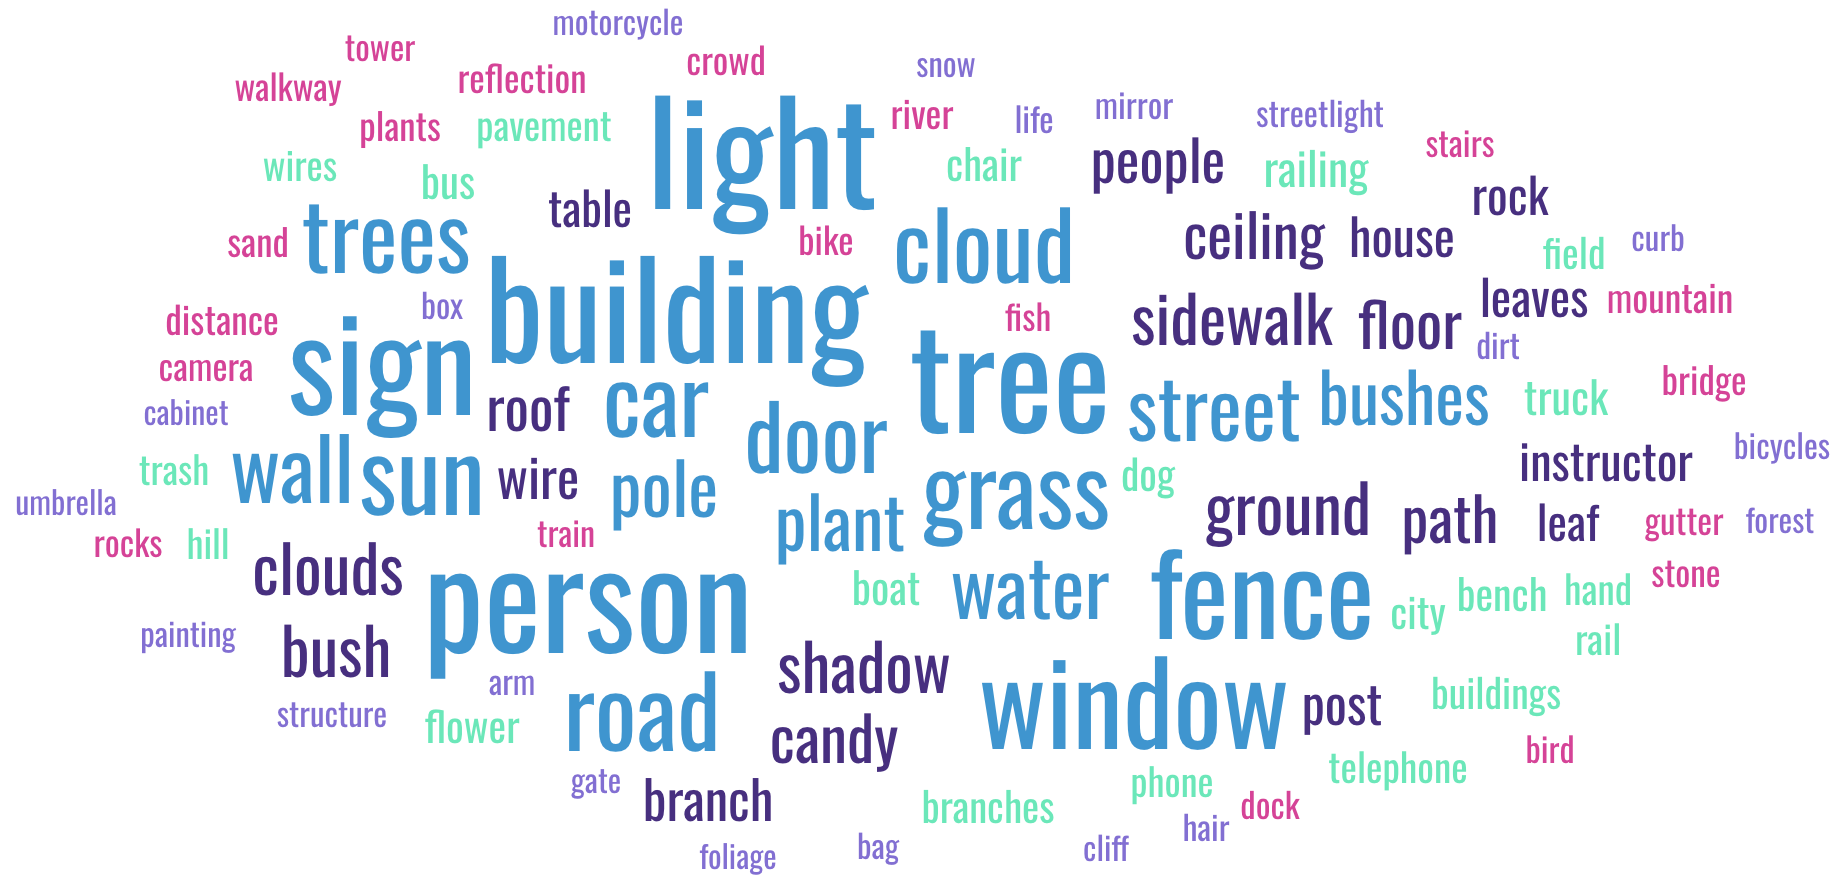
\includegraphics[width=\linewidth]{fig/wordcloud.png}
    \caption{\textbf{Diverse scene content:} A word cloud of captioned frames from our dataset shows our data is diverse, including a variety of common objects seen in videos.}
    \label{fig:wordcloud}
\end{figure}


\subsection{Stereo4D Dataset}

\Fig{motion_distribution} illustrates a subset of videos and reconstructions from a dataset processed with the above pipeline, encompassing more than 100K clips capturing everyday scenes and activities. To visualize the range of content, we used an automatic captioning system to generate captions for the dataset and created a word cloud (\Fig{wordcloud}) highlighting the most frequently observed objects.






\begin{figure}[t]
    \centering
    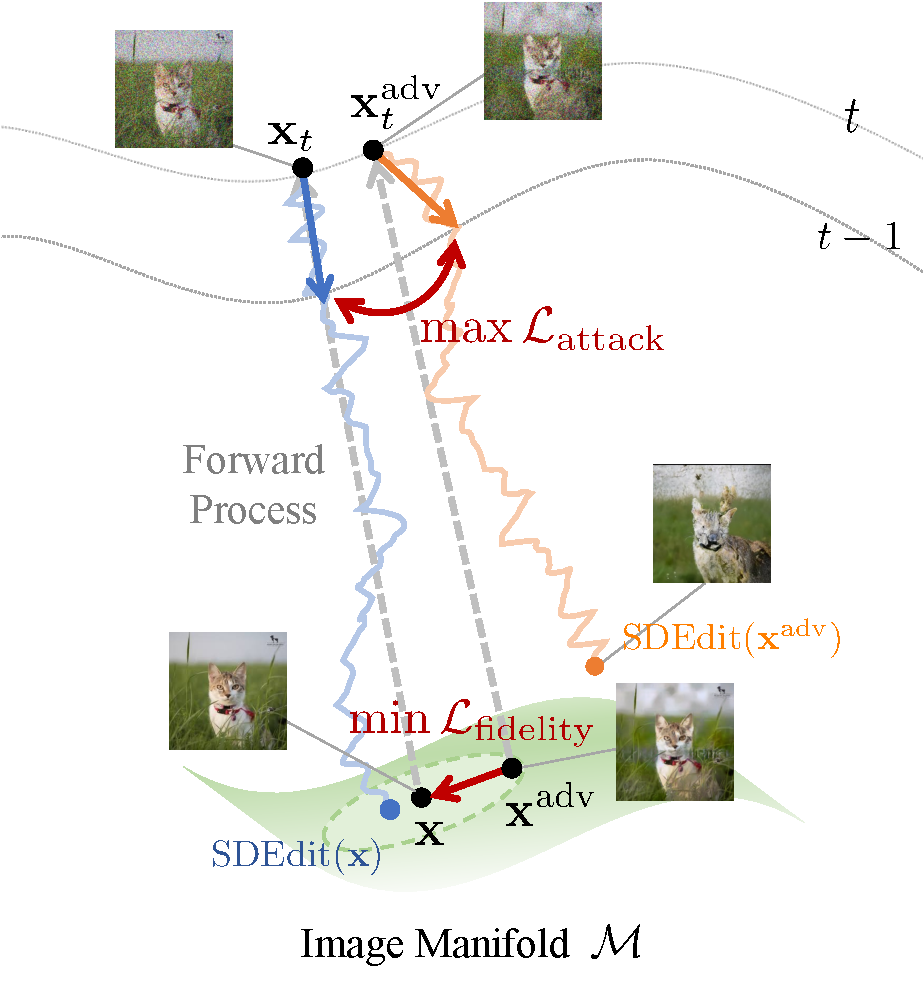
\includegraphics[width=1\linewidth]{figures/manifold.pdf}
    \caption{Conceptual illustration of our method. We randomly forward both the clean image $\mathbf{x}$ and adversarial image $\mathbf{x}^{\adv}$ to noise level $t$, then utilize our feature attacking loss to maximize the feature distance between noisy latent $\mathbf{x}_t$ and $\mathbf{x}^{\adv}_t$ in the reverse process of diffusion models while imposing our fidelity loss as a constraint to ensure the adversarial image from being deviated from the original image. We update the $\mathbf{x}^{\adv}$ in latent space instead of in pixel space to ensure the naturalness of $\mathbf{x}^{\adv}$.}
    \label{concept}
\end{figure}


\section{Methodology}

\subsection{Threat Model and Problem Setting}
The malicious user collects an image $\mathbf{x}$ from the internet and uses SDEdit \cite{meng2021sdedit} to generate unauthorized image translations or editing, denoted as $\text{SDEdit}(\mathbf{x}, t)$, that manipulates the original input image $\mathbf{x}$.

Our work aims to safeguard the input image $\mathbf{x}$ from the authorized manipulations by crafting an adversarial image $\mathbf{x}^{\adv}$ by adding imperceptible perturbation to disrupt the reverse diffusion process of SDEdit for corrupted editions.

For example, we want the main object of the image, e.g., the cat in the source image $\mathbf{x}$ as shown in Figure~\ref{concept} unable to be reconstructed by the reverse diffusion process. Meanwhile, the adversarial image should maintain similarity to the source image to ensure fidelity. The reason why we target SDEdit as our threat model is that it is recognized as the most common and general operation in diffusion-based unconditional image translations and conditional image editing. Additionally, it has been incorporated into various editing pipelines~\cite{tsaban2023leditsrealimageediting, zhang2023inversion}. Here we focus on the unconditional image translations for our main study, as they are essential in both unconditional and conditional editing pipelines. Formally, our objective to effectively safeguard images while maintaining fidelity is formulated as:

\begin{equation}
    \begin{aligned}
        & \max_{\mathbf{x}^{\adv} \in \mathcal{M}} d(\text{SDEdit}(\mathbf{x}, t), \text{SDEdit}(\mathbf{x}^{\adv}, t)) \\
    & \text{subject to } d^{\prime}(\mathbf{x}, \mathbf{x}^{\adv}) \leq \delta,
    \end{aligned}
    \label{eq:probelm_setting_constraint}
\end{equation}

where $\mathcal{M}$ indicates natural image manifold, $d$, $d^{\prime}$ indicate image distance functions and $\epsilon$ denotes the fidelity budget.

In the following sections, we first present a conceptual illustration of our method, followed by our framework for solving the optimization problem. We then discuss the novel design of our attacking loss and fidelity constraints, which provide more efficient criteria compared to previous methods for solving the image protection optimization problem using PGD. Finally, we introduce an advanced design to enhance image protection quality by latent optimization via victim-model-agnostic VAE.

\begin{figure*}[t]
    \centering
    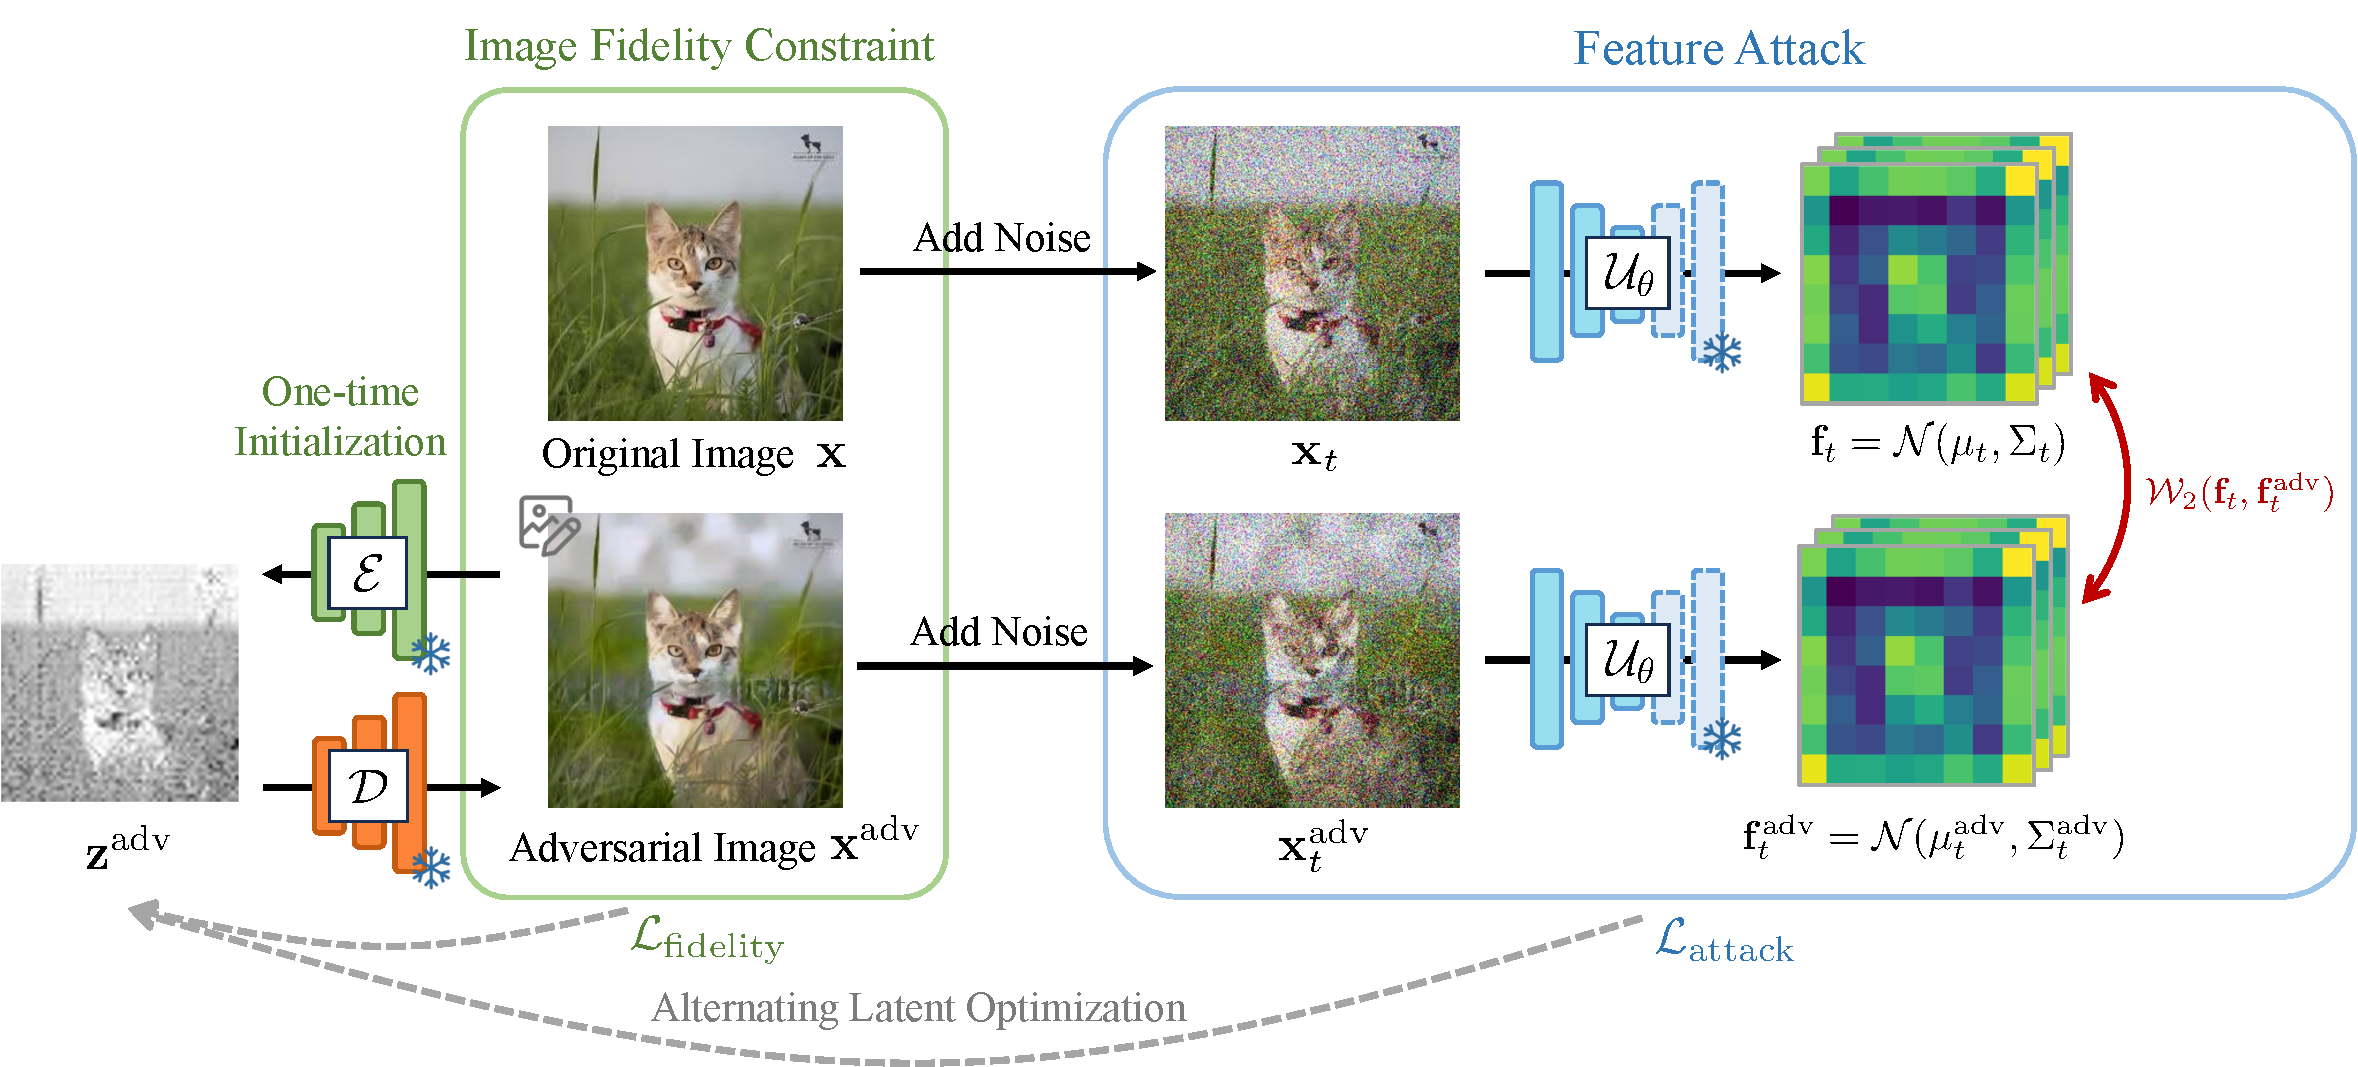
\includegraphics[width=1\linewidth]{figures/framework.pdf}
    \caption{Overview of our AtkPDM$^{+}$ algorithm: Starting from the leftmost latent of the initial adversarial image  $\mathbf{z}^{\adv}$, we first decode back to pixel-domain to perform forward diffusion with both $\mathbf{x}$ and $\mathbf{x}^{\adv}$ and feed them to frozen victim UNet. We then extract the feature representation in UNet to calculate our $\mathcal{L}_\text{attack}$, aiming to distract the recognition of image semantics. We also calculate our $\mathcal{L}_\text{fidelity}$ in pixel-domain to constrain the optimization. Finally, the $\mathbf{z}^{\adv}$ is being alternatively updated by loss gradients.}
    \label{framework}
\end{figure*}


\subsection{Overview}

To achieve effective protection against diffusion-based editing, we aim to push the protected sample away from the original clean sample by disrupting the intermediate step in the reverse diffusion process. For practical real-world applications, it's essential to ensure the protected image is perceptually similar to the original image. In practice, we uniformly sample the value of the forward diffusion step $t \sim [0, T]$ to generate noisy images and then perform optimization to craft the adversarial image $\mathbf{x}^{\adv}$ via our attacking and fidelity losses, repeating the same process $n$ times or until convergence. Figure \ref{concept} depicts these two push-and-pull criteria during different noise levels, the successful attack is reflected in the light orange line where the reverse sample moves far away from the normal edition of the image. More specifically, our method can be formulated as follows:

\begin{equation}
    \begin{aligned}
        & \max_{\mathbf{x}^{\adv} \in \mathcal{M}}
        \mathbb{E}_{
        t,
        \mathbf{x}_t| \mathbf{x}, \mathbf{x}_t^{\adv}| \mathbf{x}}
         \left[-\mathcal{L}_\text{attack}(\mathbf{x}_t, \mathbf{x}_t^{\adv})\right] \\
        & \text{subject to } \mathcal{L}_\text{fidelity}(\mathbf{x}, \mathbf{x}^{\adv}) \leq \delta,
    \end{aligned}
    \label{eq:probelm_setting_constraint}
\end{equation}

\noindent where $\delta$ denotes the attacking budget. The details of the attacking loss $\mathcal{L}_\text{attack}$ and the fidelity loss $\mathcal{L}_\text{fidelity}$ will be discussed in the following sections.


\subsubsection{Framework.}
Our framework is illustrated in Figure~\ref{framework}. We fix two identical victim UNets to extract feature representations of clean and protected samples for optimizing to push away from each other. A protection loss is jointly incorporated to constrain the optimization. After $N$ iterations, we segment out only the protecting main object of the image for better imperceptibility of image protection.

\subsection{Proposed Losses}
We propose two novel losses as optimization objectives to craft an adversarial example efficiently without running through all the diffusion steps. Attacking loss is designed to distract the feature representation in denoising UNet; Protection loss is a constraint to ensure the image quality. For notation simplicity, we first define the samples $\mathbf{x}, \mathbf{x}^{\adv}$ in different forwarded steps. 

Let $\mathcal{F}(\mathbf{x}, t, \epsilon) = \sqrt{\bar{\alpha}_t} \mathbf{x} + \sqrt{1-\bar{\alpha}_t} \epsilon$ be the diffusion forward process. Given timestep $t$ sample from $[0, T]$, noises $\epsilon_1, \epsilon_2$ sample from $\normaldist$. We denote $\mathbf{x}_t = \mathcal{F}(\mathbf{x}, t, \epsilon_1)$, and $\mathbf{x}^{\adv}_t = \mathcal{F}(\mathbf{x}^{\adv}, t, \epsilon_1)$.

\subsubsection{Attacking Loss.}
Our goal is to define effective criteria that could finally distract the reverse denoising process. PhotoGuard~\cite{salman2023raisingcostmaliciousaipowered} proposed to backpropagate through all the steps of the reverse denoising process via PGD, however, this approach is prohibitively expensive, Diff-Protect~\cite{xue2024effectiveprotectiondiffusionbased} proposed to avoid the massive cost by leveraging Score Distillation~\cite{poole2022dreamfusiontextto3dusing2d} in optimization. However, Diff-protect relies heavily on gradients of attacking encoder of an LDM as stated in their results. In PDM, we don't have such an encoder to attack; nevertheless, we find that the denoising UNet has a similar structure to encoder-decoder models, and some previous works~\cite{lin2024diffusionmodelperceptualloss, li2023fasterdiffusionrethinkingrole} characterize this property to accelerate and enhance the generation. From our observations of the feature roles in denoising UNets, we hypothesize that distracting specific inherent feature representation in UNet blocks could lead to effectively crafting an adversarial image. In practice, we first extract the feature representations of forwarded images $\mathbf{x}_t$ and $\mathbf{x}^{\adv}_t$ in frozen UNet blocks of timestep $t$. Then, we adopt 2-Wasserstein distance~\cite{arjovsky2017wasserstein} to measure the discrepancy in feature space. Note that we take the negative of the calculated distance, as we aim to pull the $\mathbf{x}^{\adv}_t$ away from $\mathbf{x}_t$. Formally, the attacking loss $\mathcal{L}_\text{attack}$ is defined as:
\begin{equation}
    \mathcal{L}_\text{attack}(\mathbf{x}_t, \mathbf{x}^{\adv}_t)
    =-\mathcal{W}_2 \left(
    \mathcal{U}^\text{(mid)}_{\theta}(\mathbf{x}_t), \mathcal{U}^\text{(mid)}_{\theta}(\mathbf{x}^{\adv}_t)
    \right).
\end{equation}

\noindent Assuming the feature distributions approximate Gaussian distributions expressed by mean $\mu_t$ and $\mu_t^{\adv}$, and non-singular covariance matrices $\Sigma_t$ and $\Sigma_t^{\adv}$. The calculation of the 2-Wasserstein distance between two normal distributions is viable through the closed-form solution~\cite{dowson1982frechet, olkin1982distance, chen2018optimal}:

\begin{equation}
    \begin{aligned}
        & \mathcal{W}_2^2(\mathcal{N}(\mu_t, \Sigma_t), \mathcal{N}(\mu_t^{\adv}, \Sigma_t^{\adv}))
        = \|\mu_t-\mu_t^{\adv}\|_2^2 \\
        & \qquad + \text{trace} (\Sigma_t + \Sigma_t^{\adv}
        -2({\Sigma_t^{\adv}}^{\frac{1}{2}}\Sigma_t{\Sigma_t^{\adv}}^{\frac{1}{2}})^\frac{1}{2} ).
    \end{aligned}
    \label{eq:wasserstein_distance}
\end{equation}

\subsubsection{Fidelity Loss.}
To control the attack budget for adversarial image quality, we design a constraint function that utilizes the feature extractor from a pretrained classifier for calculating fidelity loss. In our case, we sum up the 2-Wasserstein feature losses of $L$ different layers. Specifically, we define $\mathcal{L}_\text{fidelity}$ as:
\begin{equation}
    \mathcal{L}_\text{fidelity}(\mathbf{x}_t, \mathbf{x}^{\adv}_t)
    = \sum_{\ell=1}^L \mathcal{W}_2(\phi_\ell(\mathbf{x}), \phi_\ell(\mathbf{x}^{\adv})),
\end{equation}
where $\mathcal{W}_2$ denotes 2-Wasserstein distance and $\phi_\ell$ denotes layer $\ell$ of the feature extractor.


\subsection{Alternating Optimization for Adversarial Image}
We solve the constrained optimization problems via alternating optimization to craft the adversarial images, detailed optimization loop of AtkPDM$^{+}$ is provided in Algorithm ~\ref{alg:attdpmplus}. AtkPDM algorithm and the derivation of the alternating optimization are provided in Appendix.


\subsection{Latent Optimization via Pretrained-VAE}
Previous works suggest that diffusion models have a strong capability of resisting adversarial perturbations~\cite{xue2024pixelbarrierdiffusionmodels}, making them hard to attack via pixel-domain optimization. Moreover, they are even considered good purifiers of adversarial perturbations~\cite{nie2022diffusionmodelsadversarialpurification}. Here we propose a latent optimization strategy that crafts the ``perturbation'' in latent space. We adopt a pre-trained Variational Autoencoder (VAE) ~\cite{kingma2014autoencoding} to convert images to their latent space, and the gradients will be used to update the latent, after N iterations or losses converge, we decode back via decoder $\mathcal{D}$ to pixel domain as our final protected image. The motivation for adopting VAE is inspired by MPGD~\cite{he2024manifold}. This strategy is effective for crafting a robust adversarial image against pixel-domain diffusion models while also better preserving the protection quality rather than only incorporating fidelity constraints. The constraint optimization thereby becomes: 
\begin{equation}
\begin{aligned}
    & \max_{\mathbf{z}^{\adv}}
    \mathbb{E}_{
    t,
    \mathbf{x}_t| \mathbf{x}, \mathbf{x}_t^{\adv}| \mathcal{D}(\mathbf{z}^{\adv})}
    \left[-\mathcal{L}_\text{attack}(\mathbf{x}_t, \mathbf{x}_t^{\adv})\right] \\
    & \text{subject to } \mathcal{L}_\text{fidelity}(\mathbf{x}, \mathcal{D}(\mathbf{z}^{\adv})) \leq \delta.
\end{aligned}
\label{eq:probelm_setting_constraint}
\end{equation}

\noindent Detailed latent optimization loop is provided in Algorithm~\ref{alg:attdpmplus}.


\begin{algorithm}[t]
    \caption{AtkPDM$^{+}$}
    \label{alg:attdpmplus}
    \small{
    \begin{algorithmic}[1] 
        \STATE{\textbf{Input:}
        Image to be protected $\mathbf{x}$, attack budget $\delta > 0$, step size $\gamma_1, \gamma_2>0$, \textcolor{black}{VAE encoder $\mathcal{E}$, and VAE decoder $\mathcal{D}$}}
        \STATE{\textbf{Initialization:} $\mathbf{x}^{\adv} \leftarrow \mathbf{x}$, $L_\text{attack} \leftarrow \infty$}
        \STATE{\textcolor{black}{Encode adversarial image to latent space: $\mathbf{z}^{\adv} \leftarrow \mathcal{E}(\mathbf{x}^{\adv})$}}
        \WHILE{$L_\text{attack}$ not convergent}
            \STATE{\textcolor{black}{Decode adversarial latent to pixel space: $\mathbf{x}^{\adv} \leftarrow \mathcal{D}(\mathbf{z}^{\adv})$}}
            \STATE{Sample timestep: $t \sim [0, T]$}
            \STATE{Sample noise: $\epsilon_1, \epsilon_2 \sim \normaldist$}
            \STATE{Compute original noisy sample: $\mathbf{x}_t \leftarrow \mathcal{F}(\mathbf{x}, t, \epsilon_1)$}
            \STATE{Compute adversarial noisy sample: $\mathbf{x}^{\adv}_t \leftarrow \mathcal{F}(\mathbf{x}^{\adv}, t, \epsilon_2)$}
            \STATE{\textcolor{black}{Update $\mathbf{z}^{\adv}$ by Gradient Descent: \\
            $\mathbf{z}^{\adv} \leftarrow \mathbf{z}^{\adv} -
            \gamma_1 \sign(\nabla_{\mathbf{z}^{\adv}} \mathcal{L}_\text{attack}(\mathbf{x}_t, \mathbf{x}^{\adv}_t))$}}
            \WHILE{$\mathcal{L}_\text{fidelity}(\mathbf{x}, \textcolor{black}{\mathcal{D}(\mathbf{z}^{\adv})}) > \delta$}
            \STATE{ 
            \textcolor{black}{$\mathbf{z}^{\adv} \leftarrow \mathbf{z}^{\adv} -
            \gamma_2 \nabla_{\mathbf{z}^{\adv}} \mathcal{L}_\text{fidelity}(\mathbf{x}, \mathcal{D}(\mathbf{z}^{\adv}))$}}
            \ENDWHILE
        \ENDWHILE
        \STATE{\textcolor{black}{Decode adversarial latent to pixel space: $\mathbf{x}^{\adv} \leftarrow \mathcal{D}(\mathbf{z}^{\adv})$}}
        \RETURN {$\mathbf{x}^{\adv}$}
    \end{algorithmic}
    }
\end{algorithm}


\section{Experiment Results}
In this section, we examine the attack effectiveness and robustness of our approach under extensive settings. 



\begin{table*}[t]
    \centering
    \small{
    \begin{tabular}{ll|ccc|cccc}
        \toprule
        & \multirow{2}{*}{Methods} & \multicolumn{3}{c|}{Adversarial Image Quality} & \multicolumn{4}{c}{Attacking Effectiveness} \\ 
         & & SSIM $\uparrow$ & PSNR $\uparrow$ & LPIPS $\downarrow$ & SSIM $\downarrow$ & PSNR $\downarrow$ & LPIPS $\uparrow$ & IA-Score $\downarrow$ \\
        \midrule
        \multirow{4}{*}{\rotatebox{90}{Church}}
        & PGAscent & 0.37 $\pm$ 0.09 & 28.17 $\pm$ 0.22 & 0.73 $\pm$ 0.16 & 0.89 $\pm$ 0.05 & 31.06 $\pm$ 1.94 & 0.17 $\pm$ 0.09 & 0.93 $\pm$ 0.04 \\
        & Diff-Protect & 0.39 $\pm$ 0.07 & 28.03 $\pm$ 0.12 & 0.67 $\pm$ 0.11 & 0.82 $\pm$ 0.05 & 31.90 $\pm$ 1.08 & 0.23 $\pm$ 0.07 & 0.91 $\pm$ 0.04 \\
        & AtkPDM (Ours) & \second{0.75} $\pm$ 0.03 & \second{28.22} $\pm$ 0.10 & \second{0.26} $\pm$ 0.04 & \first{0.75} $\pm$ 0.04 & \first{29.61} $\pm$ 0.23 & \first{0.40} $\pm$ 0.05 & \first{0.76} $\pm$ 0.06 \\
        & atkPDM$^+$ (Ours) & \first{0.81} $\pm$ 0.03 & \first{28.64} $\pm$ 0.19 & \first{0.13} $\pm$ 0.02 & \second{0.79} $\pm$ 0.04 & \second{30.05} $\pm$ 0.47 & \second{0.33} $\pm$ 0.07 & \second{0.81} $\pm$ 0.06 \\
        \midrule
        \multirow{4}{*}{\rotatebox{90}{Cat}}
        & PGAscent & 0.48 $\pm$ 0.09 & 28.34 $\pm$ 0.18 & 0.65 $\pm$ 0.12 & 0.96 $\pm$ 0.02 & \second{32.32} $\pm$ 2.49 & 0.10 $\pm$ 0.05 & 0.97 $\pm$ 0.03 \\
        & Diff-Protect & 0.33 $\pm$ 0.10 & 28.03 $\pm$ 0.15 & 0.80 $\pm$ 0.15 & \second{0.90} $\pm$ 0.05 & 33.94 $\pm$ 1.93 & \second{0.18} $\pm$ 0.08 & 0.95 $\pm$ 0.03 \\
        & atkPDM (Ours) & \second{0.71} $\pm$ 0.06 & \second{28.47} $\pm$ 0.18 & \second{0.29} $\pm$ 0.05 & \first{0.83} $\pm$ 0.03 & \first{30.73} $\pm$ 0.51 & \first{0.39} $\pm$ 0.05 & \first{0.81} $\pm$ 0.04 \\
        & atkPDM$^+$ (Ours) & \first{0.83} $\pm$ 0.04 & \first{29.41} $\pm$ 0.37 & \first{0.09} $\pm$ 0.02 & 0.93 $\pm$ 0.01 & 33.02 $\pm$ 0.74 & \second{0.18} $\pm$ 0.02 & \second{0.92} $\pm$ 0.01\\
        \midrule
        \multirow{4}{*}{\rotatebox{90}{Face}}
        & PGAscent & 0.48 $\pm$ 0.05 & \first{28.75} $\pm$ 0.18 & 0.64 $\pm$ 0.10 & 0.99 $\pm$ 0.00 & 37.96 $\pm$ 1.75 & 0.02 $\pm$ 0.01 & 0.99 $\pm$ 0.00 \\
        & Diff-Protect  & 0.25 $\pm$ 0.04 & 28.09 $\pm$ 0.20 & 0.91 $\pm$ 0.11 & 0.95 $\pm$ 0.02 & 35.33 $\pm$ 1.62 & 0.08 $\pm$ 0.04 & 0.96 $\pm$ 0.02 \\
        & atkPDM (Ours) & \second{0.56} $\pm$ 0.04 & 28.01 $\pm$ 0.22 & \second{0.36} $\pm$ 0.04 & \first{0.74} $\pm$ 0.03 & \first{29.14} $\pm$ 0.36 & \first{0.40} $\pm$ 0.05 & \first{0.62} $\pm$ 0.07 \\
        & atkPDM$^+$ (Ours) & \first{0.81} $\pm$ 0.04 & \second{28.39} $\pm$ 0.20 & \first{0.12} $\pm$ 0.03 & \second{0.86} $\pm$ 0.03 & \second{30.26} $\pm$ 0.72 & \second{0.24} $\pm$ 0.07 & \second{0.80} $\pm$ 0.08 \\
        \bottomrule
    \end{tabular}
    }
    \caption{Quantitative Results in attacking different PDMs. The best is marked in red and the second best is marked in blue. Errors denote one standard deviation of all images in our test datasets.}
    \label{tab:attackPDM}
    \vspace*{-10pt}
\end{table*}




\begin{table}[t]
\footnotesize{
    \centering
    \begin{tabular}{lcccc}
        \toprule
        \multirow{2}{*}{Defense Method} & \multicolumn{4}{c}{Attacking Effectiveness} \\ 
         &  SSIM $\downarrow$ & PSNR $\downarrow$ & LPIPS $\uparrow$ & IA-Score $\downarrow$ \\
        \midrule
        Crop-and-Resize & 0.68 & 29.28 & 0.42 & 0.79 \\
        JPEG Comp. & 0.78  & 29.82 & 0.36 & 0.79 \\
        \midrule
        None & 0.79 & 30.05 & 0.33 & 0.81 \\
        \bottomrule
    \end{tabular}
    \caption{Quantitative results of our adversarial images against defense methods. Both Crop-and-Resize and JPEG Compression fail to defend our attack. ``None'' indicates no defense is applied, as the baseline for comparison.}
    % The term "None" in the defense method column indicates the use of the adversarial image generated by our method without applying any purification techniques.
\label{tab:defense}
}
\end{table}



\subsection{Experiment Settings}
\subsubsection{Implementation Details.} We conduct all our experiments in white box settings and examine the effectiveness of our attacks using SDEdit \cite{meng2021sdedit}. For the Variational Autoencoder (VAE) ~\cite{kingma2014autoencoding} in our AtkPDM$^{+}$, we utilize the VAE provided by StableDiffusion V1.5 ~\cite{rombach2022high}.
We run all of our experiments with 300 optimization steps, which is empirically determined, to balance attacking effectiveness and image protection quality with reasonable speed. Other loss parameters and running time are provided in the Appendix. The implementation is built on the Diffusers library. All the experiments are conducted with a single Nvidia Tesla V100 GPU.


\subsubsection{Victim Models and Datasets.}
We test our approach on PDMs with three open-source checkpoints on HuggingFace, specifically ``google/ddpm-ema-church-256'', ''google/ddpm-cat-256'' and ``google/ddpm-ema-celebahq-256''. For the results reported in Table~\ref{tab:attackPDM}, we run 30 images for each victim model. Additionally, for generalizability in practical scenarios, we synthesize the data with half randomly from the originally trained dataset and another half from randomly crawled with keywords from the Internet.

\subsubsection{Baseline Methods and Evaluation Metrics.}

To the best of our knowledge, previous methods have mainly focused on LDMs, and effective PDM attacks have not yet been developed, however, we still implement Projected Gradient Ascent (PGAscent) with their proposed semantic loss by~\cite{salman2023raisingcostmaliciousaipowered, liang2023adversarialexampledoesgood, liang2023mistimprovedadversarialexamples, xue2024effectiveprotectiondiffusionbased}. Notably, Diff-Protect~\cite{xue2024effectiveprotectiondiffusionbased} proposed to minimize the semantic loss is surprisingly better than maximizing the semantic loss, we also adopted this method in attacking PDMs and denote as Diff-Protect. To quantify the adversarial image visual quality, we adopted Structural Similarity (SSIM) ~\cite{wang2004image}, Peak Signal-to-Noise Ratio (PSNR), and Learned Perceptual Image Patch Similarity (LPIPS) ~\cite{zhang2018unreasonable}. We also inherit these three metrics, but negatively to quantify the effectiveness of our attack. We also adopted Image Alignment Score (IA-Score) \cite{kumari2023multi} that leverages CLIP \cite{radford2021learning} to calculate the cosine similarity of image encoder features. In distinguishing from previous methods, to more faithfully reflect the attack effectiveness, we fix the same seed of the random generator when generating clean and adversarial samples, then calculate the scores based on the paired samples.

\subsection{Attack Effectiveness on PDMs}

As quantitatively reported in Table~\ref{tab:attackPDM} and qualitative results in Figure~\ref{qualitative}, compared to previous PGD-based methods incorporating semantic loss, i.e., negative training loss of diffusion models, our method exhibits superior performance in both adversarial image quality and attacking effectiveness. And our reported figures has generally stable as reflected in lower standard deviation. It is worth noting that even if the adversarial image qualities of the PGD-based methods are far worse than ours, their attacking effectiveness still falls short, suggesting that PDMs are robust against traditional perturbation methods, this finding is also aligned with previous works~\cite{xue2024effectiveprotectiondiffusionbased,xue2024pixelbarrierdiffusionmodels}. For AtkPDM$^+$, combined with our latent optimization strategy, the adversarial image quality has enhanced while slightly affecting the attacking effectiveness, still outperforming the previous methods.



\begin{table}[t]
\footnotesize{
    \centering
    \begin{tabular}{lcccc}
        \toprule
        \multirow{2}{*}{Setting} & \multicolumn{4}{c}{Attacking Effectiveness} \\ 
         &  SSIM $\downarrow$ & PSNR $\downarrow$ & LPIPS $\uparrow$ & IA-Score $\downarrow$ \\
        \midrule
        White Box & 0.79 & 30.05 & 0.33 & 0.81 \\
        
        Black Box & 0.86 & 30.25 & 0.29 & 0.85 \\
    
        \midrule
        Difference & 0.07 & 0.20 & 0.04 & 0.04 \\
        \bottomrule
    \end{tabular}
    \caption{Quantitative results of black box attack. We use the same set of adversarial images and feed to white box and black box models to examine the black box transferability.} 
\label{tab:blackBox}
}
\end{table}
\begin{figure*}[t]
\centering
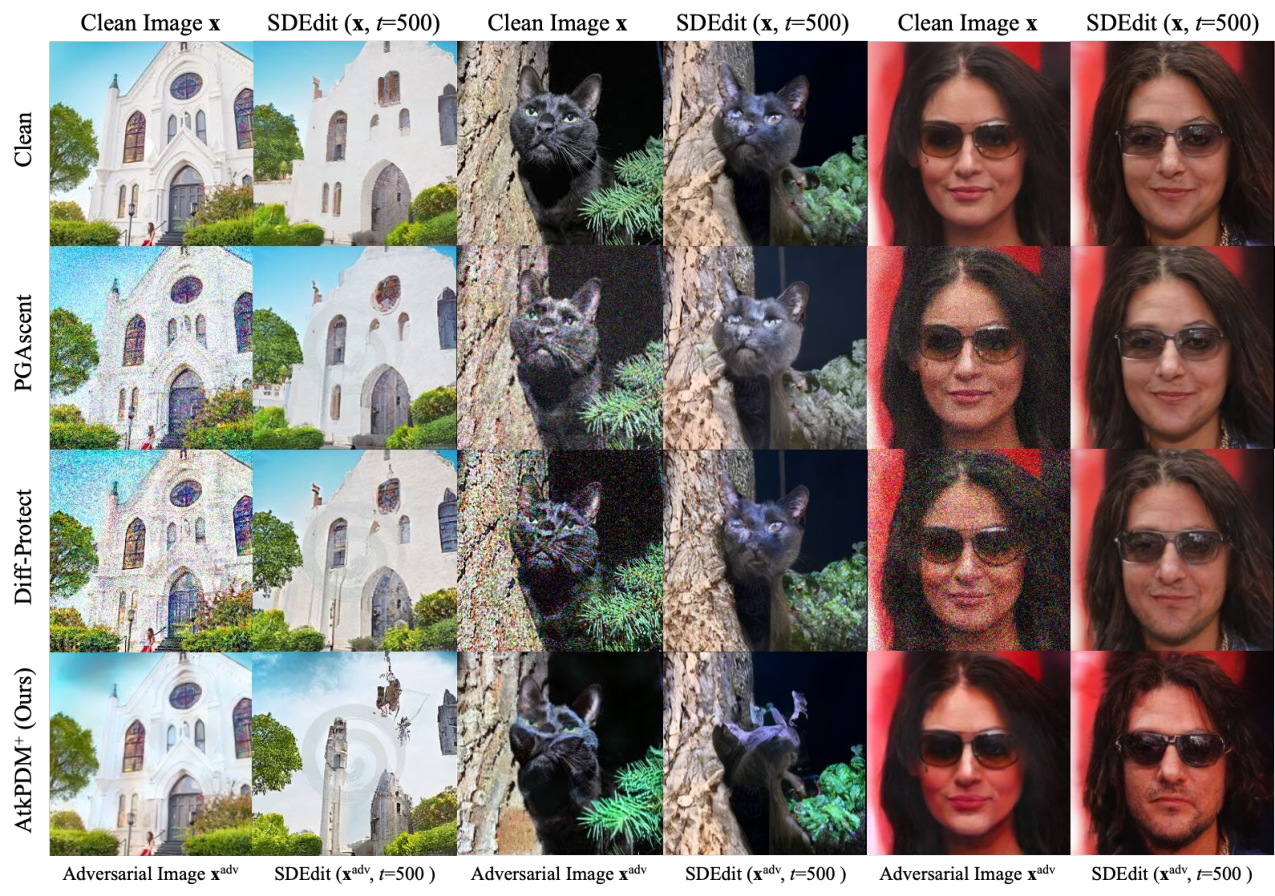
\includegraphics[width=0.79\linewidth]{figures/qualitative_results.pdf}
\caption{Qualitative results compared to previous methods: our adversarial images can effectively corrupt the edited results without significant fidelity decrease. The same column shares the same random seed for fair comparison.
}
\label{qualitative}
\end{figure*}

\begin{table*}
    \centering
    \small{
    \begin{tabular}{lc|ccc|cccc}
        \toprule
        \multirow{2}{*}{Losses} & \multirow{2}{*}{VAE} & \multicolumn{3}{c|}{Adversarial Image Quality} & \multicolumn{4}{c}{Attacking Effectiveness} \\ 
         & & SSIM $\uparrow$ & PSNR $\uparrow$ & LPIPS $\downarrow$ & SSIM $\downarrow$ & PSNR $\downarrow$ & LPIPS $\uparrow$ & IA-Score $\downarrow$ \\
        \midrule
        $\mathcal{L}_\text{semantic}$ &  & 0.37 $\pm$ 0.09  & 28.17 $\pm$ 0.22 & 0.73 $\pm$ 0.16  & 0.89 $\pm$ 0.05 & 31.06 $\pm$ 1.94 & 0.17 $\pm$ 0.09 & 0.93 $\pm$ 0.04 \\
        $\mathcal{L}_\text{semantic}$ & \checkmark & 0.80 $\pm$ 0.05 & \second{29.78} $\pm$ 0.42 & \second{0.17} $\pm$ 0.03 & 0.82 $\pm$ 0.05 & 30.43 $\pm$ 0.75 & 0.15 $\pm$ 0.06 & 0.92 $\pm$ 0.04 \\
        % $\mathcal{L}_\text{semantic}$ + $\mathcal{L}_\text{fidelity}$ &  & 0.12  & 27.90 & 1.08 & \first{0.58} & \first{28.01} & \first{0.93} & \first{0.61} \\ 
        $\mathcal{L}_\text{semantic}$ + $\mathcal{L}_\text{fidelity}$ & \checkmark & \first{0.82} $\pm$ 0.05 & \first{30.30} $\pm$ 0.81 & \first{0.13} $\pm$ 0.03 & 0.90 $\pm$ 0.03 & 31.24 $\pm$ 1.19 & 0.08 $\pm$ 0.03 & 0.96 $\pm$ 0.02 \\
        \midrule
        $\mathcal{L}_\text{attack}$ + $\mathcal{L}_\text{fidelity}$ (Ours) & & 0.75 $\pm$ 0.03 & 28.22 $\pm$ 0.10  & 0.26 $\pm$ 0.04 & \first{0.75} $\pm$ 0.04 & \first{29.61} $\pm$ 0.23 & \first{0.40} $\pm$ 0.05 & \first{0.76} $\pm$ 0.06 \\
        $\mathcal{L}_\text{attack}$ + $\mathcal{L}_\text{fidelity}$ (Ours) & \checkmark & \second{0.81} $\pm$ 0.03 & 28.64 $\pm$ 0.19 & \first{0.13} $\pm$ 0.02 & \second{0.79} $\pm$ 0.04 & \second{30.05} $\pm$ 0.47 & \second{0.33} $\pm$ 0.07 & \second{0.81} $\pm$ 0.06 \\
        \bottomrule
    \end{tabular}
    }
    \caption{Quantitative results of ablation study. The best is in bold and the second best is underlined. Errors denote one standard deviation of all images in our test datasets.}
    \label{tab:loss_ablation}
    \vspace*{-10pt}
\end{table*}



\subsection{Against Defense Methods}
We examine the robustness of our approach against two widely recognized and effective defense methods for defending against adversarial attacks as reported in Table~\ref{tab:defense}.

\subsubsection{Crop and Resize.}
Noted by Diff-Protect, crop and resize is simple yet the most effective defense method against their attacks on LDMs. We also test our method against this defense using their settings, i.e., cropping 20\% of the adversarial image and then resizing it to its original dimensions.


\subsubsection{JPEG Compression.}
Sandoval-Segura et al.~\cite{sandoval2023jpeg} demonstrated that JPEG compression is a simple yet effective adversarial defense method. In our experiments, we implement the JPEG compression at a quality setting of 25\%. The quantitative results in Table~\ref{tab:defense} demonstrate that our method is robust against these two defense methods, with four of the metrics listed in Table~\ref{tab:defense} are not worse than no defenses. Surprisingly, these defense methods even make the adversarial image more effective than cases without defense.


\subsection{Black Box Transferability}
We craft adversarial images with the proxy model, ``google/ddpm-ema-church-256'', in white-box settings and test their transferability to another ``google/ddpm-bedroom-256'' model for black-box attacks. Under identical validation settings, Table~\ref{tab:blackBox} reveals only a slight decrease in attack effectiveness metrics, indicating successful black-box transferability.



\subsection{Effectiveness of Latent Optimization via VAE}
We first incorporate our VAE latent optimization strategy in the previous semantic-loss-based PGAscent. From Table~\ref{tab:loss_ablation}, without using $\mathcal{L}_\text{fidelity}$, latent optimization has significantly enhanced the adversarial image quality and even slightly improved the attacking effectiveness. Adopting latent optimization in our approach enhances visual quality with a negligible decrease in attacking effectiveness. Surprisingly, incorporating our $\mathcal{L}_\text{fidelity}$ with current PGD-based method will drastically decrease the adversarial image quality despite its attack performing better than ours. This may be due to different constrained optimization problem settings.

\section{Discussion and Conclusion}
\noindent \textbf{Limitations.} 
Our data curation pipeline and trained model have limitations. 
The quality of the long-range 3D motion tracks depends on the accuracy of optical flow and 2D point tracking and may degrade for distant background regions or objects occluded for long periods.
Additionally, \method is a non-generative model that only operates on two-frame inputs. 
Extending our model to video input by adopting an extra global optimization~\cite{zhang2024monst3r} or integrating generative priors for modeling ambiguous motion content is a promising future direction.

\bfpar{Conclusion.}
We presented a pipeline for mining high-quality 4D data from Internet stereoscopic videos. Our framework automatically annotates each real-world video sequence with camera parameters, 3D point clouds, and long-range 3D motion trajectories by consolidating different noisy structure and motion estimates derived from videos.  Furthermore, we show that training a variant of \duster on our real-world 4D data enables more accurate learning of 3D structure and motion in dynamic scenes, outperforming other baselines.



{
    \small
    \bibliographystyle{ieeenat_fullname}
    \bibliography{main}
}

% WARNING: do not forget to delete the supplementary pages from your submission 
\clearpage

\setcounter{page}{1}
\maketitlesupplementary

% \section{Supplementary video}
% Please see the supplementary video for an overview of our paper and for additional visualizations.

\section{\dataset Statistics}
We collected around 110k clips from 6,493 Internet VR180 videos.
\Fig{supp:camera_stats} shows the camera translation distribution between the first and last frame of each clip. 
In \Fig{supp:motion_stats}, we measure the motion in terms of pixel displacement projected onto the image frame. Measuring motion in pixel-space emphasizes motion that occurs closer to the camera, since such motion yields larger pixel displacements, while naturally de-emphasizing motion further from the camera. 

\section{More qualitative comparisons}
% Please see the supplementary video for additional visual examples of data in \dataset.


\subsection{More results on held-out  \dataset examples}
\Fig{supp:qualitative-stereo4d} shows additional \method predictions on the \dataset held-out test set, extending \Fig{result-wall-stereo4dtest} from the main paper. \Fig{supp:compare-stereo4d} shows additional qualitative examples of motion comparisons on \dataset test set, extending~\Fig{compare-stereo4d} from the main paper. \Fig{supp:compare-stereo4d} compares variants of DynaDUSt3R trained on different data sources. The model trained on PointOdyssey incorrectly predicts large 3D motions, while the model trained on Stereo4D makes more accurate motion predictions, closer to ground truth.

\begin{figure}[t]
    \centering
    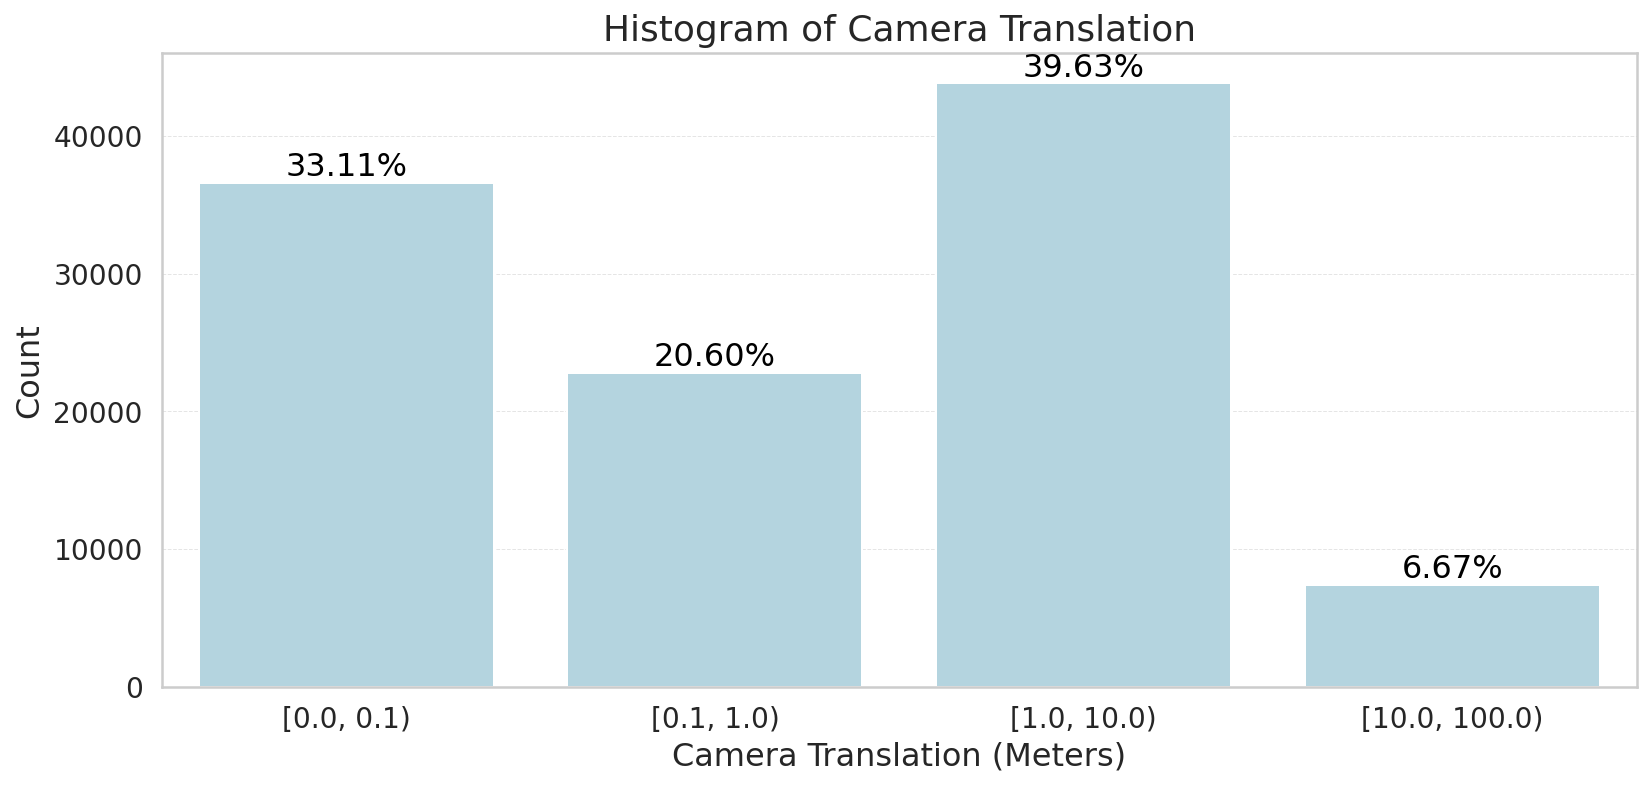
\includegraphics[width=\linewidth]{fig/supp/camera_stats.png}
    \caption{Camera statistics from \dataset. We measure the difference (in meters) of camera poses between the start and end frame of each video clip as calculated by SfM.}
    \label{fig:supp:camera_stats}

    \centering
    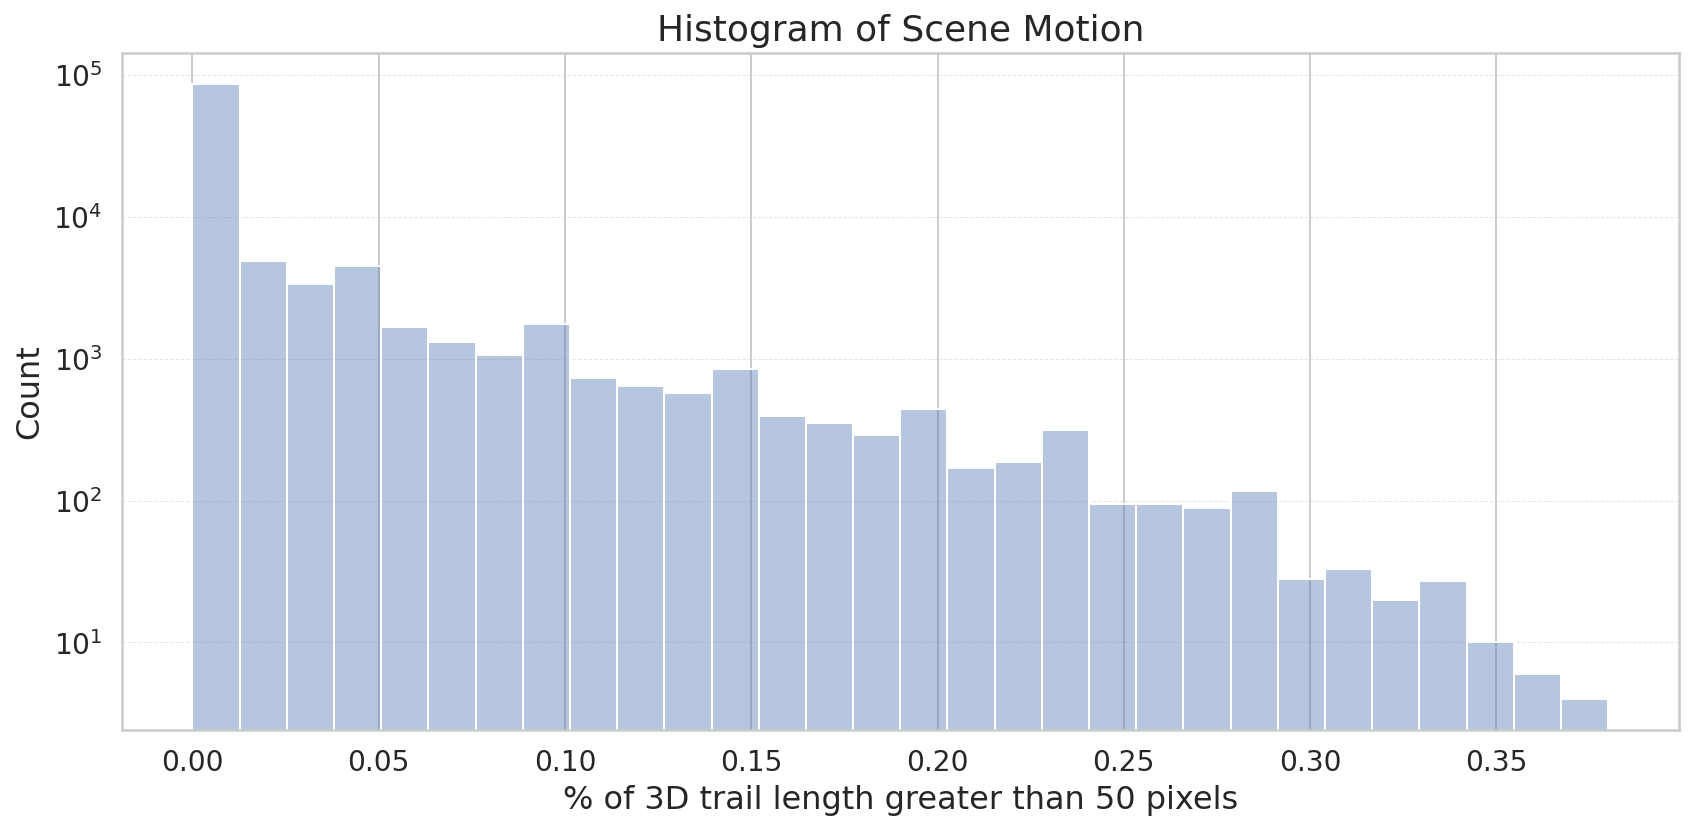
\includegraphics[width=\linewidth]{fig/supp/track_stats.png}
    \caption{Scene motion statistics from \dataset. We measure the motion in terms of pixel displacement projected onto the image frame. For each video, we measure the percentage of tracks that have 3D trail length greater than 50 pixels. The 3D trail length is measured by Eqn.~\ref{eqn:trail_length_def}. }
    \label{fig:supp:motion_stats}
\end{figure}

\begin{figure*}[ht]
    \centering
    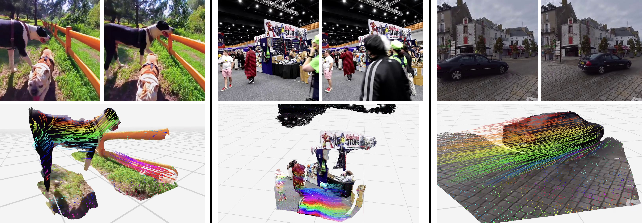
\includegraphics[width=\textwidth]{fig/supp/qualitative-stereo4d.pdf}
    \caption{\textbf{More qualitative results on \dataset test set.} Extending~\Fig{result-wall-stereo4dtest}, we visualize image pairs and corresponding dynamic 3D point clouds predicted by DynaDUSt3R trained on \dataset. Our method recovers accurate 3D shape and complex scene motion.}
\label{fig:supp:qualitative-stereo4d}
\end{figure*}

\begin{figure*}[ht]
    \centering
    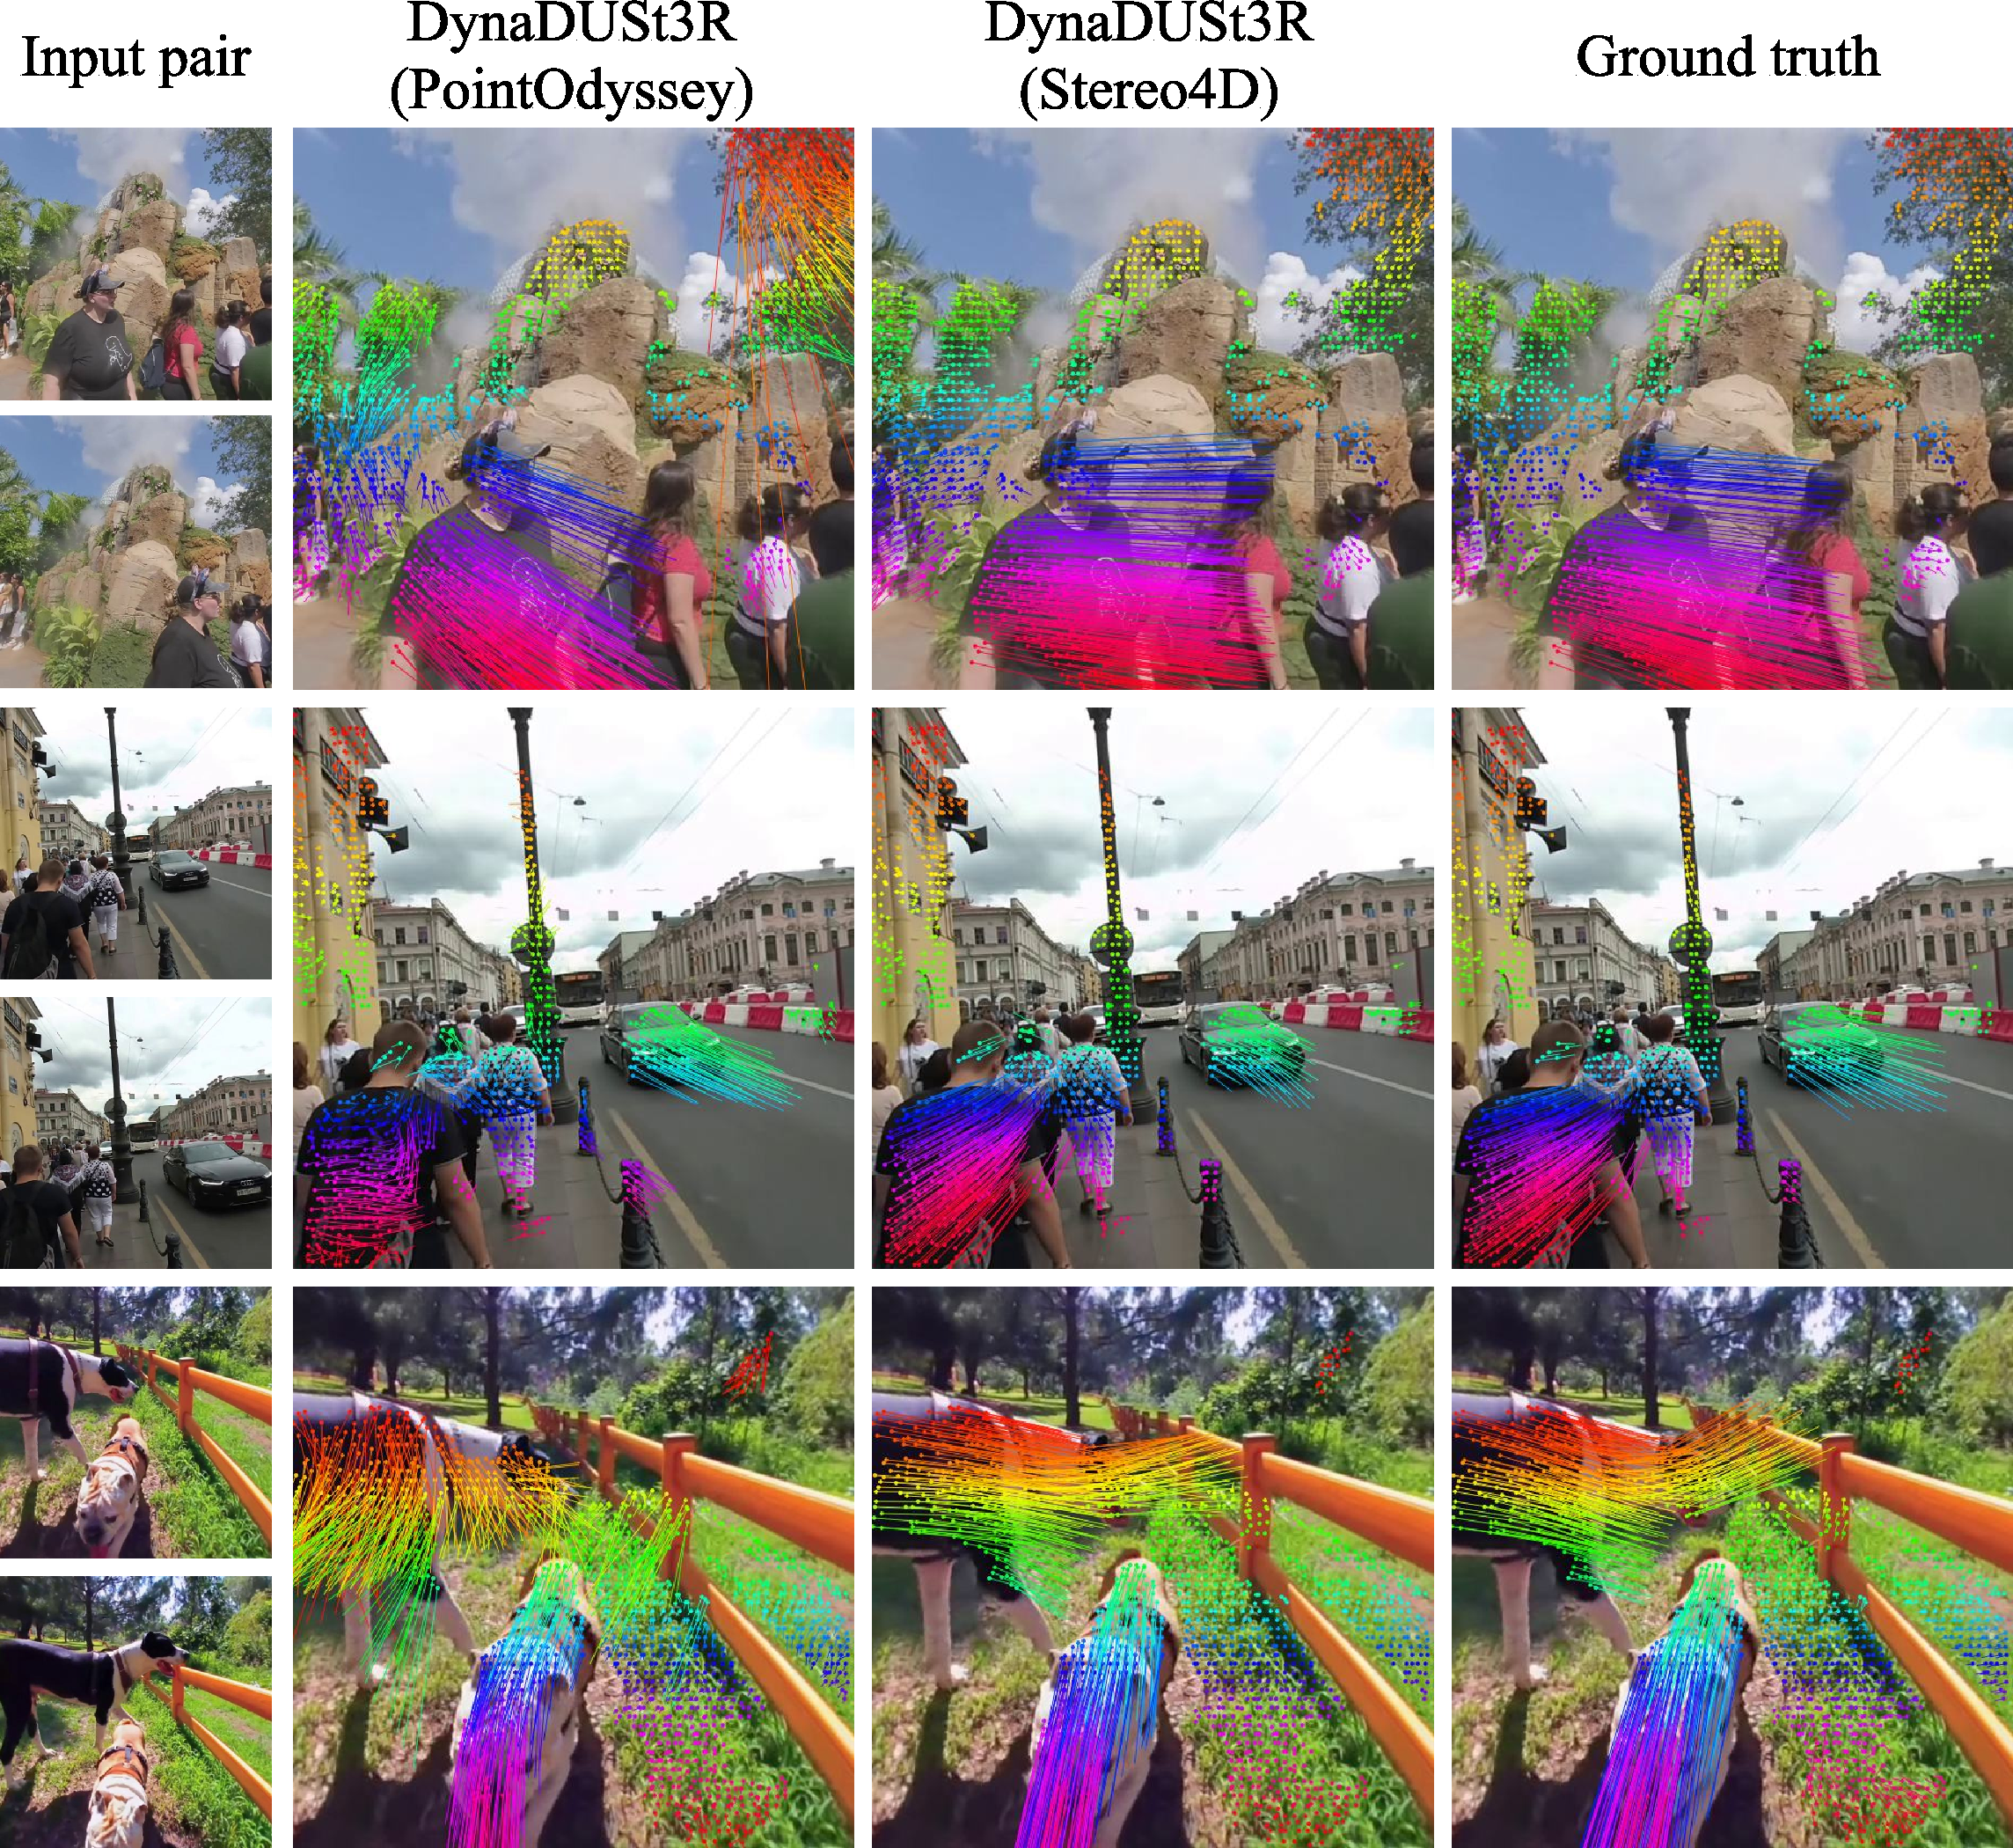
\includegraphics[width=\textwidth]{fig/supp/qualitative_comparison_on_motion_stereo4d.pdf}
    \caption{\textbf{More qualitative comparisons of 3D motion in the \dataset test set.} Extending~\Fig{compare-stereo4d}, we compare variants of DynaDUSt3R trained on different data sources. The Stereo4D-trained model also makes more precise motion predictions than the PointOdyssey-trained model.}
\label{fig:supp:compare-stereo4d}
\end{figure*}



\subsection{More qualitative examples on track optimization}
In \Fig{supp:track_comparison}, we illustrate estimated tracks for a video sequence featuring a forward-moving camera and vehicles driving towards the camera. Our initial 3D tracks derived directly from RAFT depth, BootsTAP 2D tracks, and SfM camera pose, show significant jitter for both dynamic (vehicle) and static (ground) points. 
However, after applying our track optimization, the ground points produce stable, static tracks, and vehicle tracks become smooth and coherent. 

\begin{figure*}[ht]
    \centering
    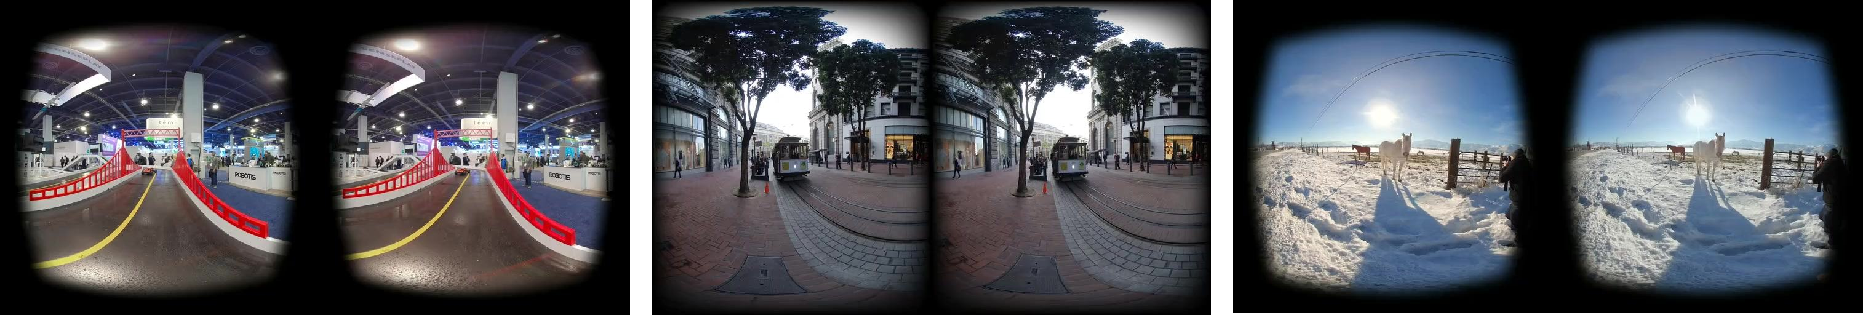
\includegraphics[width=\textwidth]{fig/supp/equirect-sample.pdf}
    \caption{Example equirectangular stereo videos collected from the internet.}
    \label{fig:supp:equirect}
\end{figure*}


\begin{figure*}[ht]
    \centering
    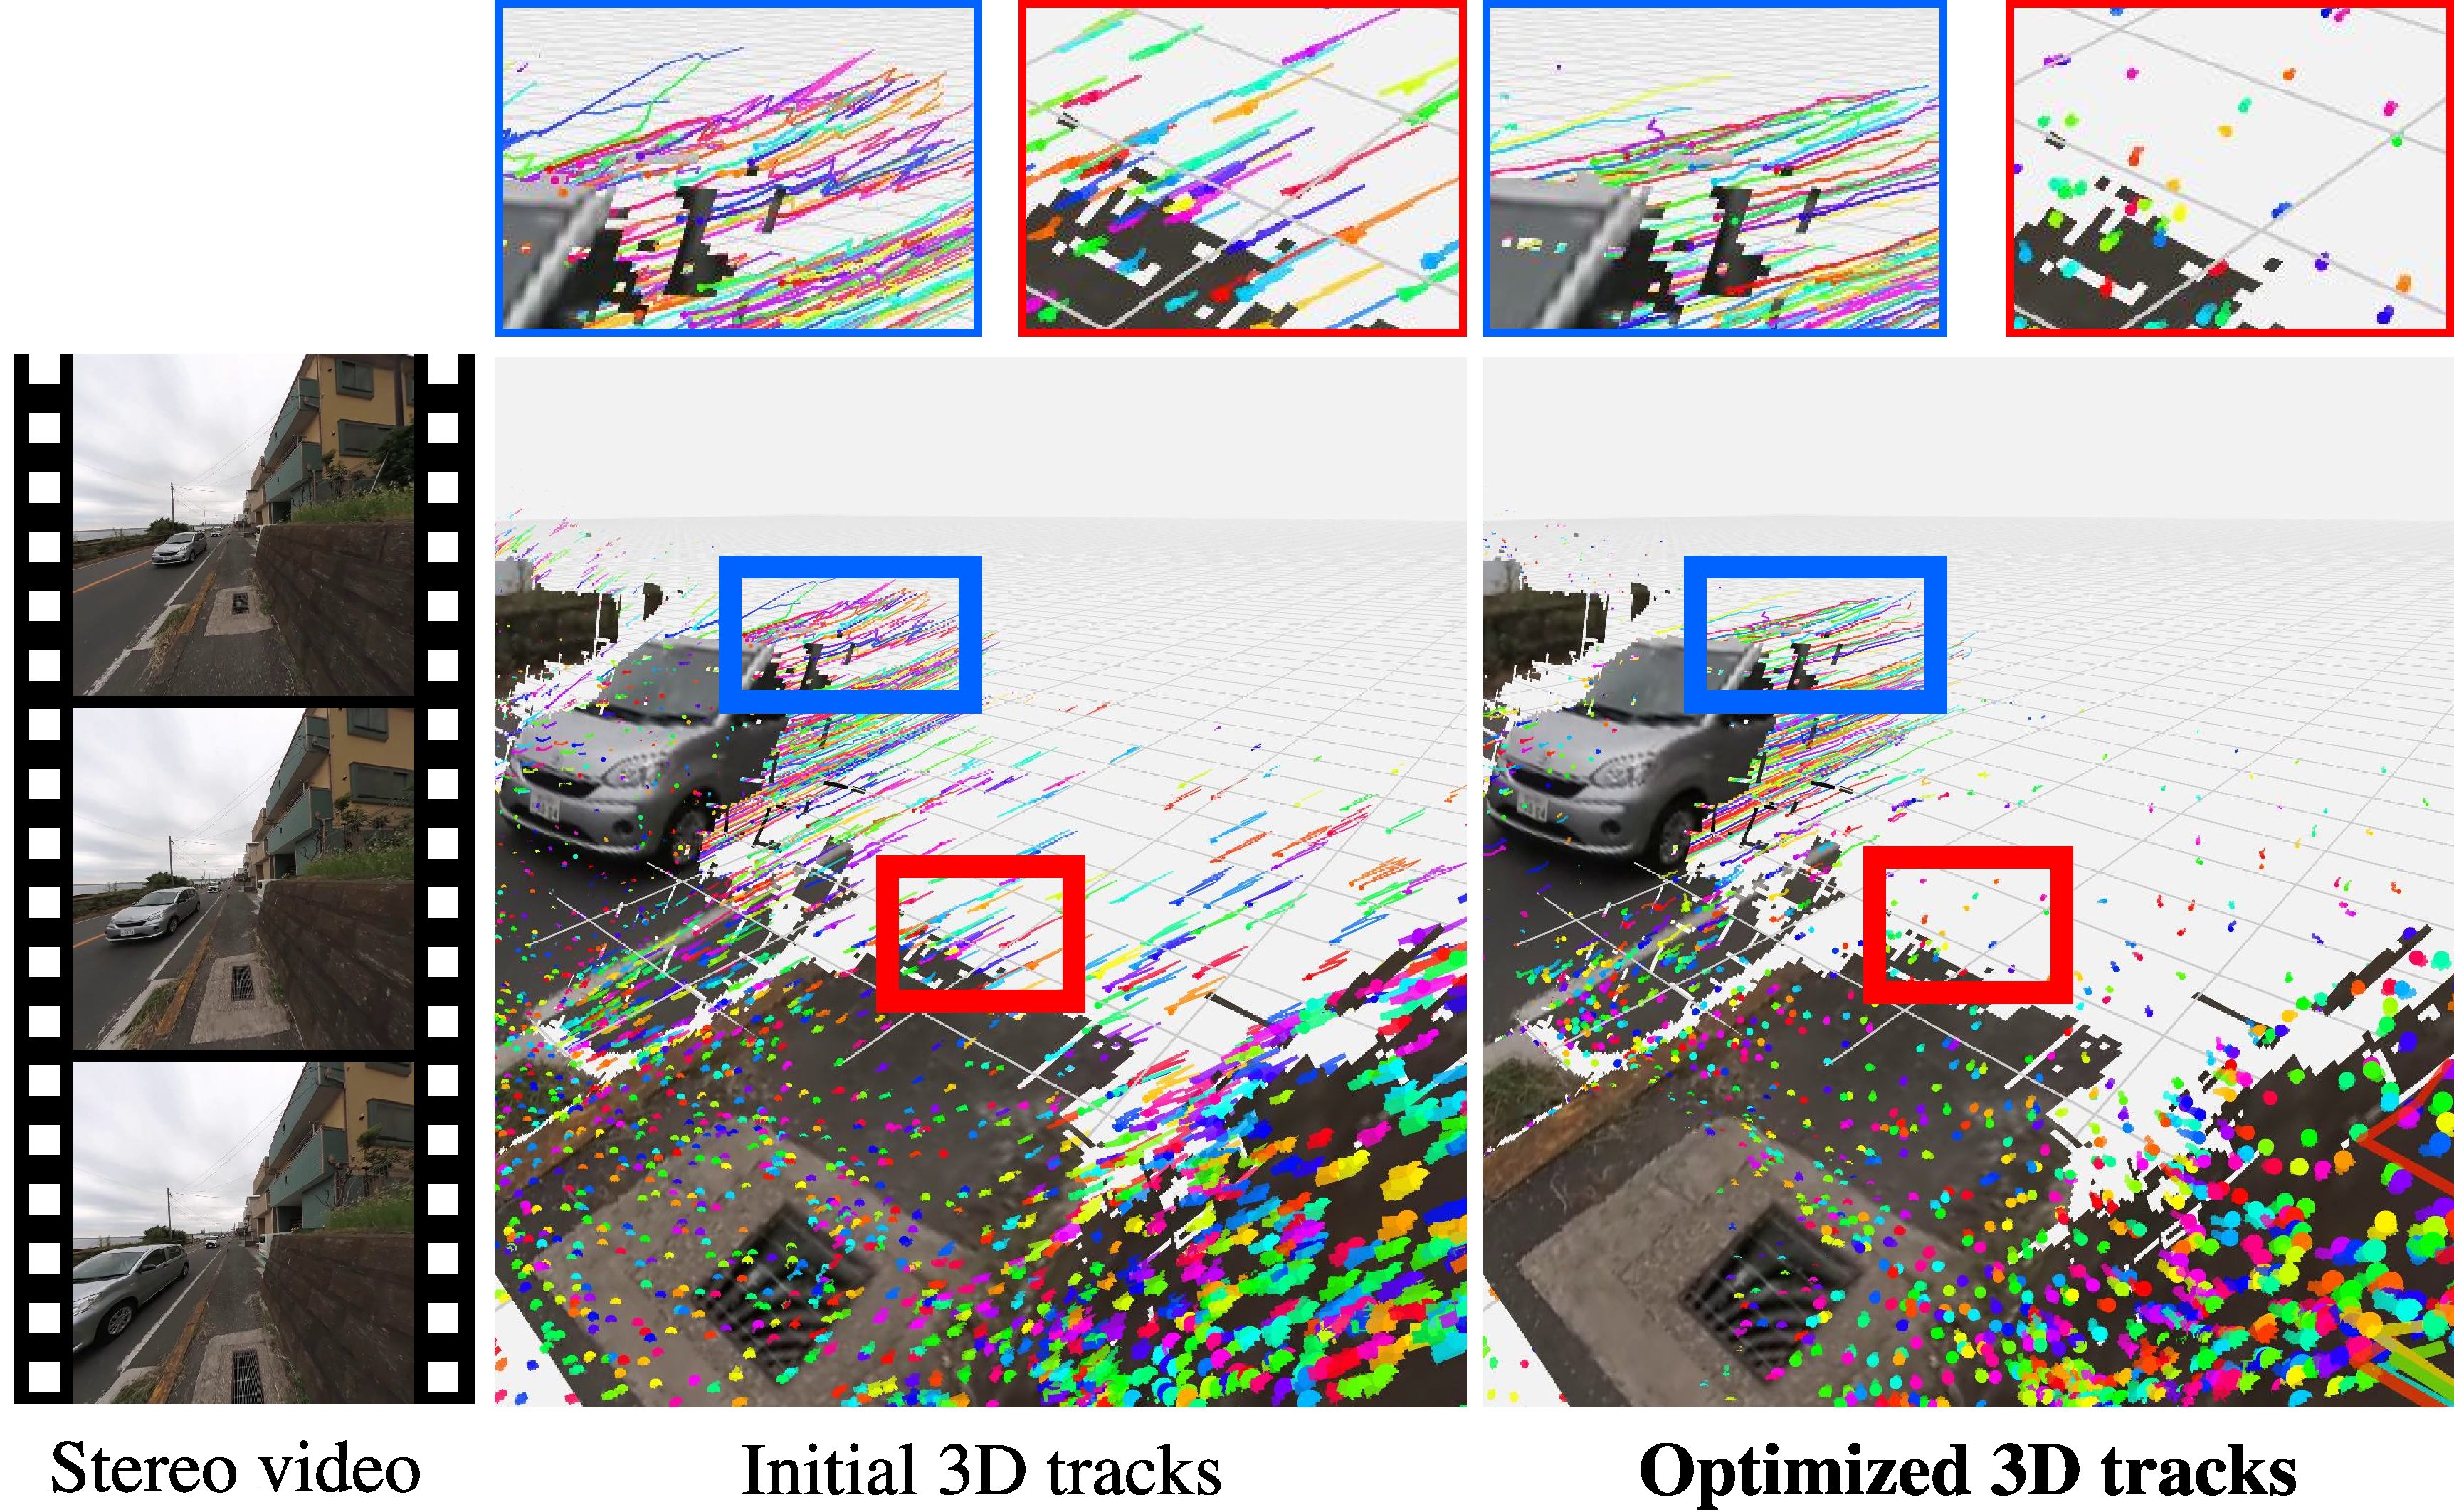
\includegraphics[width=0.8\textwidth]{fig/supp/track_optimization_car_comparison-2.pdf}
    \caption{\textbf{Effect of Track Optimization.} We compare 3D tracks on a challenging walking tour video sequence. In this clip (left), the camera moves forward while vehicles drive toward the camera. We visualize the results across 16 frames, showing 3D trails left by both dynamic and static points.  \textbf{Middle}: Our initial 3D tracks, created directly from RAFT, BootsTAP and SfM camera pose, also exhibit significant jitter for both dynamic (vehicle) and static (ground) points.  \textbf{Right}: After applying our track optimization, the ground points yield stable, static tracks, and vehicle tracks become smooth and coherent.}
\label{fig:supp:track_comparison}
\end{figure*}

\section{Dataset curation details}
\subsection{Equirectangular videos}
The raw videos that we collect (see examples in \Fig{supp:equirect}) are natively stored in a cropped equirectangular format, which differs from a full 360$^\circ$ equirectangular projection as the horizontal field of view of the cropped format typically spans 180$^\circ$---half of a full sphere. These videos often contain metadata specifying the horizontal and vertical field of view. 
For instance, metadata for a typical video might specify 
$\mathsf{start_{yaw}}=-90.0^\circ$, $\mathsf{end_{yaw}}=90.0^\circ$,  $\mathsf{start_{tilt}}=-90.0^\circ$, $\mathsf{end_{tilt}}=90.0^\circ$; 
Since many VR180 videos are designed for an immersive VR experience, they are typically viewed with headsets. Hence, the baseline between the left and right cameras typically closely matches the average human eye distance of 6.3 cm.


\subsection{SfM}
For ease of processing with standard 3D computer vision pipelines, and to benefit from the wide FoV of the input videos, we convert the videos from their native format (equirectangular projections) to a fisheye format for camera pose estimation. 
We use a 140$^\circ$ field of view for these fisheye-projected videos, because many equirectangular videos have a black fade-out/feathering/vignetting effect applied at the boundary, as shown in~\Fig{supp:equirect}.
We found that using wider FoV frames significantly improves camera pose estimation in dynamic scenes. 
When using narrow FoV projections, dynamic objects are more likely to occupy a large fraction of the frame; when these dynamic foreground objects are rich in features, they can confuse camera tracking algorithms, leading to inaccurate camera poses that track the dynamic object rather than producing true camera motion with respect to the environment. 
In contrast, wide-angle fisheye videos capture more background regions, which tend to have stable features for tracking, yielding more reliable camera poses.

We first use ORB-SLAM2's stereo estimation mode~\cite{murartal2015orbslam}
to identify trackable sequences within the videos, utilizing the method devised by Zhou \etal to divide videos into discrete, trackable shots~\cite{zhou2018stereo}. 
For each given shot, consisting of frames $(I_i, \ldots, I_n)$, we estimate camera poses and rig calibration via an incremental global bundle adjustment algorithm similar to COLMAP~\cite{schonberger2016structure}. 
We initialize the stereo rig calibration to be that of a rectified stereo pair with baseline 6.3 cm, but optimize for the calibration as part of the bundle adjustment process, as in practice the stereo rig can vary significantly from its nominal configuration.
This process yields a camera position $\mathbf{c}_i$ and orientation $\mathbf{R}_i$ for each frame $i$ (defined as the pose of the left camera), and a position $\mathbf{c}_r$ and orientation $\mathbf{R}_r$ for the right camera relative to the left (assumed to be constant throughout the shot).


\subsection{Depth estimation}
Depth estimation is first performed on a per-frame basis, with disparity maps computed independently for each frame.  

We use the estimated camera rig calibration $\cB_r, \RB_r$ to rectify the original  high resolution equirectangular video frames, ensuring that (1) the left and right views have centered principal points, (2) are oriented perpendicular to the baseline, and (3) pointing in a parallel direction.  We then convert the equirectangular videos to  perspective projections for downstream predictions.

Disparity is estimated from optical flow~\cite{teed2020raft, sun2022disentangling} between the rectified left and right frames. 
The $x$-component of the optical flow is used as disparity, which is converted to metric depth using:
\begin{equation}
    \mathsf{Depth} = \frac{\mathsf{baseline}  \times f}{\mathsf{disparity}}.
\end{equation}
Here $\mathsf{baseline}=0.063$m, and $f$ is the frame's focal length.

\medskip
\noindent \textbf{Outlier Rejection.} Several criteria are applied to filter out unreliable pixels: \emph{Inconsistency between left and right eyes:} Disparity is rejected if the optical flow fails a cycle-consistency check with an error exceeding one pixel. \emph{Depth values exceeding 20 meters} are considered invalid. Estimating accurate depth beyond a certain range requires sub-pixel disparity estimation, and therefore the resulting depths are usually very noisy.
\emph{Negative flow values} that shouldn't occur, but can, often due to errors in textureless regions.
\emph{Large vertical flow:} pixels with a y-component of flow exceeding one pixel are removed (as in our rectified stereo pairs correspondences should have the same $y$-value, and violating that epipolar constraint indicates uncertain matches).
\emph{Occlusion boundaries:} Depth gradients exceeding a threshold ($\mathsf{threshold} = 0.3$) indicate occlusion boundaries and are rejected. For a pixel location $(x, y)$, depth gradients are computed as:
$$\mathsf{grad_x}=|{\mathsf{Depth}(x+1, y)-\mathsf{Depth}(x-1,y)} |,$$ $$\mathsf{grad_y}=|{\mathsf{Depth}(x, y+1)-\mathsf{Depth}(x,y-1)} |.$$
Pixels are rejected if $\mathsf{grad_x} > \mathsf{threshold} \times \mathsf{Depth}(x,y)$ or  $\mathsf{grad_y} > \mathsf{threshold} \times \mathsf{Depth}(x,y)$.

\subsection{2D tracks}
We extract long-range 2D point trajectories using BootsTAP~\cite{doersch2024bootstap}. 
We run tracking on the left-eye video only. 
For every 10 frames, we uniformly initialize query points on image with stride 4. We then remove duplicated queries if earlier tracks fall within 1 pixel of a query point.

\subsection{Choice of FoV and resolution for perspective projection.}
When converting the equirectangular videos to perspective projections, we use two FoVs: 60$^\circ$ and 120$^\circ$. Both perspective videos are set to a resolution of $512\times512$, the maximum supported by BootsTAP. The 60$^\circ$ projection offers a higher sampling rate in scene units, which improves the accuracy of depth estimation and 2D tracks when measured in meters. Additionally, it has smaller perspective distortion near the image boundaries. In contrast, the $120^\circ$ projection provides wider coverage, ensuring longer 2D tracks across the videos. This trade-off allows us to balance data quality with spatial coverage for downstream tasks, e.g. \method. We take the union of the 3D tracks derived from each of these videos for \method training supervision.

\section{\method training details.}
\bfpar{Dataloader.} During training, we randomly sample two frames from the training videos that are at most 60 frames apart, at times $t_0$ and $t_1$, ($t_0 < t_1$). 
Additionally, we also sample one auxiliary frame in between, at time $t_{\mathsf{aux}}, t_0<t_\mathsf{aux}<t_1$, for additional track supervision between the two input frames. During training, we add data augmentation by applying random crops and color jitter to the input images and cropping the ground truth pointmap and motionmap accordingly. 

\bfpar{Training.} The network takes input the two RGB images as well as query times $t_q = \{0, 1, \frac{t_\mathsf{aux}-t_0}{t_1-t_0}\}$ and predicts the pointmaps for the two input views and motionmaps for each query $t_q$.
We supervise the network with losses defined in Eqn.~\ref{eqn:loss_point} and \ref{eqn:loss_motion}. We initialize our network with the \duster weights and initialize the motion head with the same weights as the point head. We finetune for 49k iterations with batch size 64, learning rate $2.5\times 10^{-5}$, and optimized by Adam with weight decay 0.95. 





\end{document}
